\documentclass[twoside]{book}

\newcommand\docyear{2017 }
\newcommand\docrev{Revision F }
\newcommand\docref{SPEC98T17 }
\newcommand\docdate{07/16/2017 }
\newcommand\docstatus{CONFIDENTIAL }
\newcommand\docwarning{MAXIM INTEGRATED CONFIDENTIAL/DISTRIBUTE ONLY UNDER NDA }

% Packages required by doxygen
\usepackage{fixltx2e}
\usepackage{calc}
\usepackage{doxygen}
\usepackage[export]{adjustbox} % also loads graphicx
\usepackage{graphicx}
\usepackage[utf8]{inputenc}
\usepackage{makeidx}
\usepackage{multicol}
\usepackage{multirow}
\PassOptionsToPackage{warn}{textcomp}
\usepackage{textcomp}
\usepackage[nointegrals]{wasysym}
\usepackage[table]{xcolor}

% Font selection
%\usepackage[T1]{fontenc}
\usepackage{mathptmx}
%\usepackage[scaled=.90]{times}
%\usepackage{courier}
\usepackage{amssymb}
\usepackage{sectsty}
%\renewcommand{\familydefault}{\sfdefault}
\allsectionsfont{%
  \fontseries{bc}\selectfont%
  \color{darkgray}%
}
\renewcommand{\DoxyLabelFont}{%
  \fontseries{bc}\selectfont%
  \color{darkgray}%
}
\newcommand{\+}{\discretionary{\mbox{\scriptsize$\hookleftarrow$}}{}{}}

% Page & text layout
\usepackage{geometry}
\geometry{%
  a4paper,%
  top=2.5cm,%
  bottom=2.5cm,%
  left=2.5cm,%
  right=2.5cm%
}
\tolerance=750
\hfuzz=15pt
\hbadness=750
\setlength{\emergencystretch}{15pt}
\setlength{\parindent}{0cm}
\setlength{\parskip}{3ex plus 2ex minus 2ex}
\makeatletter
\renewcommand{\paragraph}{%
  \@startsection{paragraph}{4}{0ex}{-1.0ex}{1.0ex}{%
    \normalfont\normalsize\bfseries\SS@parafont%
  }%
}
\renewcommand{\subparagraph}{%
  \@startsection{subparagraph}{5}{0ex}{-1.0ex}{1.0ex}{%
    \normalfont\normalsize\bfseries\SS@subparafont%
  }%
}
\makeatother

% Headers & footers
\usepackage{fancyhdr}
\fancypagestyle{plain}{
\fancyhf{}
\fancyhead[L]{\raisebox{-0.5\height}{
\includegraphics[scale=0.5]{../../res/maxim-logo-202.png}}}
\fancyhead[R]{\textbf{\textit{$projectname}}}
\fancyfoot[L]{\textit{\docrev}}
\fancyfoot[R]{\fancyplain{}{\docstatus | Maxim Integrated Products Inc. | \thepage}}
}

\pagestyle{plain}

\renewcommand{\headrulewidth}{0pt}
\renewcommand{\footrulewidth}{2pt}
\renewcommand{\chaptermark}[1]{%
  \markboth{#1}{}%
}
\renewcommand{\sectionmark}[1]{%
  \markright{\thesection\ #1}%
}

\setlength{\headheight}{37pt}
\setlength{\headsep}{1.3cm}
\setlength{\topmargin}{-1.9cm}
\setlength{\footskip}{1cm}
\setlength{\textheight}{24.7cm}

% Indices & bibliography
\usepackage{natbib}
\usepackage[titles]{tocloft}
\setcounter{tocdepth}{3}
\setcounter{secnumdepth}{5}
\makeindex

% Hyperlinks (required, but should be loaded last)
\usepackage{ifpdf}
\ifpdf
  \usepackage[pdftex,pagebackref=true]{hyperref}
\else
  \usepackage[ps2pdf,pagebackref=true]{hyperref}
\fi
\hypersetup{%
  colorlinks=true,%
  linkcolor=blue,%
  citecolor=blue,%
  unicode%
}

% Custom commands
\newcommand{\clearemptydoublepage}{%
  \newpage{\pagestyle{empty}\cleardoublepage}%
}

\usepackage{caption}
\captionsetup{labelsep=space,justification=centering,font={bf},singlelinecheck=off,skip=4pt,position=top}

%CUSTOMIZATION
%

\let\cleardoublepage\clearpage
\let\oldchapter\chapter
\let\oldsection\section
\let\oldsubsection\subsection
\let\oldsubsubsection\subsubsection

\newcommand\mysection\oldsubsection
\newcommand\mysubsection\oldsubsubsection
\newcommand\mysubsubsection\paragraph
\newcommand\mysectionh\oldchapter
\newcommand\mysubsectionh\oldsection
\newcommand\mysubsubsectionh\oldsubsection

\newcommand\shiftleveldown{%
\makeatletter%
\renewcommand{\section}{\mysection}%
\renewcommand{\subsection}{\mysubsection}%
\renewcommand{\subsubsection}{\mysubsubsection}%
\makeatother%
}

\newcommand\restorelevel{%
\makeatletter%
\renewcommand{\section}{\oldsection}%
\renewcommand{\subsection}{\oldsubsection}%
\renewcommand{\subsubsection}{\oldsubsubsection}%
\makeatother%
}


\newcommand\shiftlevelup{%
\makeatletter%
\renewcommand{\section}{\mysectionh}%
\renewcommand{\subsection}{\mysubsectionh}%
\renewcommand{\subsubsection}{\mysubsubsectionh}%
\makeatother%
}

\usepackage{titlesec}

 \titleformat{\chapter}
   {\Large\bfseries} % format
   {\thechapter. }                % label
   {0pt}             % sep
   {}           % before-code

%===== C O N T E N T S =====


\begin{document}

% Titlepage & ToC
\hypersetup{pageanchor=false,
             bookmarksnumbered=true,
             pdfencoding=unicode
            }
%\pagenumbering{alph}
\begin{titlepage}
\vspace*{7cm}
\begin{flushleft}
\begin{figure}[H]

\includegraphics[scale=1]{../../res/maxim-logo-header.png}
\end{figure}
\textbf{\Large{\bf{$projectname}\\}}
\textbf{\\\docref\\}
\textbf{\docrev\\}
\textbf{\docdate\\}
\end{flushleft}

\vspace*{7cm}
\begin{flushright}
Maxim Integrated, Inc.\\
160 Rio Robles\\
San Jose, CA 95134\\
\end{flushright}

\end{titlepage}

\section*{Disclaimer}

\subsection*{LIFE SUPPORT POLICY}
MAXIM’S PRODUCTS ARE NOT AUTHORIZED FOR USE AS CRITICAL COMPONENTS IN LIFE SUPPORT DEVICES OR SYSTEMS WITHOUT THE EXPRESS PRIOR WRITTEN APPROVAL OF THE PRESIDENT AND GENERAL COUNSEL OF MAXIM INTEGRATED PRODUCTS, INC. 

\subsection*{As used herein}
Life support devices or systems are devices which (a) are intended for surgical implant into the body, or (b) support or sustain life and whose failure to perform when properly used in accordance with instructions for use provided in the labeling can be reasonably expected to result in a significant injury to the user. A critical component is any component in a life support device or system whose failure to perform can be reasonably expected to cause the failure of the life support device or system or to affect its safety or effectiveness.

\subsection*{Document Disclaimer}
©\docyear by Maxim Integrated, Inc. All rights reserved. Information in this publication concerning the devices, applications, or technology described is intended to suggest possible uses and may be superseded. MAXIM INTEGRATED, INC. DOES NOT ASSUME LIABILITY FOR OR PROVIDE A REPRESENTATION OF ACCURACY OF THE INFORMATION, DEVICES, OR TECHNOLOGY DESCRIBED IN THIS DOCUMENT. MAXIM ALSO DOES NOT ASSUME LIABILITY FOR INTELLECTUAL PROPERTY INFRINGEMENT RELATED IN ANY MANNER TO USE OF INFORMATION, DEVICES, OR TECHNOLOGY DESCRIBED HEREIN OR OTHERWISE. The information contained within this document has been verified according to the general principles of electrical and mechanical engineering or registered trademarks of Maxim Integrated, Inc. All other product or service names are the property of their respective owners. 

ARM® and Thumb® are registered trademarks of ARM Limited in the European Union and other countries. All other product or service names are the property of their respective owners.


\clearemptydoublepage
\pagenumbering{roman}
\tableofcontents
\clearemptydoublepage
\pagenumbering{arabic}
\hypersetup{pageanchor=true}

%--- Begin generated contents ---

\chapter{Document details}

\hypertarget{_r_e_l_e_a_s_e__n_o_t_e_s_rn}{}\section{Release Notes}\label{_r_e_l_e_a_s_e__n_o_t_e_s_rn}
\tabulinesep=1mm
\begin{longtabu} spread 0pt [c]{*{3}{|X[-1]}|}
\hline
\rowcolor{\tableheadbgcolor}\textbf{ Revision }&\textbf{ Date }&\textbf{ Description  }\\\cline{1-3}
\endfirsthead
\hline
\endfoot
\hline
\rowcolor{\tableheadbgcolor}\textbf{ Revision }&\textbf{ Date }&\textbf{ Description  }\\\cline{1-3}
\endhead
A &04/12/2016 &Initial Release \\\cline{1-3}
B &03/01/2017 &Add Debug Box~\newline
Refine interrupt handling discussion~\newline
Introduce event management~\newline
 Refine key management \\\cline{1-3}
C &02/02/2017 &Clarifications in the security architecture description \\\cline{1-3}
D &19/05/2017 &Reflect latest modifications \\\cline{1-3}
E &19/06/2017 &Improvements, see note 1 below \\\cline{1-3}
F &16/07/2017 &Addition of security guidelines \\\cline{1-3}
\end{longtabu}


Note 1\+: Revision E improvements vs v1.\+1 UL release

mbed-\/\+OS improvements\+:
\begin{DoxyItemize}
\item Addition of M\+A\+X32552 support \& rework of file layout in target/ folder
\item Non security related bug fixes in Maxim drivers and performance improvements.
\item Rework of the linker file to adapt to separate box signature mechanism
\item Some adjustments in the Maxim startup files
\end{DoxyItemize}

u\+Visor\textquotesingle{}s improvements\+:
\begin{DoxyItemize}
\item Upgrade from 0.\+26.\+2-\/24 to 0.\+27
\item Support for separate box signature (see related section in the main documentation)
\item New A\+PI to get signing key of a box (hence it\textquotesingle{}s privilege)
\item Support for M\+A\+X32552
\item Fix of Makefiles for correct multiple target support
\item Improvement of debug messages in the debug version
\item Add hook to implement A\+CL verification and enforcement at box loading time depending on signing key
\item Add handling of N\+MI faults
\end{DoxyItemize}

Deeptrust A\+PI\textquotesingle{}s improvements\+:

Globally\+:
\begin{DoxyItemize}
\item Support for separate box signature
\item Reorganize folders
\item Isolate crypto buffers
\item Add key manager \& crypto services
\item Separation between core firmware, firmware level boxes, trusted boxes, and other boxes
\end{DoxyItemize}

P\+CI services\+:
\begin{DoxyItemize}
\item Addition of a watchdog to automatically clear the P\+IN if not used
\item Forcibly flush the P\+IN after use
\item Keep crypto working buffer private (used to be visible from several boxes)
\item Erase buffers containing sensitive data after use\+: data\+\_\+hash.\+data\+\_\+val, issuer\+\_\+public\+\_\+key
\item Other minor bug fixes
\end{DoxyItemize}

Secure Sandbox services\+:
\begin{DoxyItemize}
\item Add a trace capability to catch security issues, and capability to add user handling for such events
\item Add secure R\+TC control
\item Add automatic reset every 24h
\item Evolutions in keypad handling and display following M\+A\+X32552 support addition
\item Buffers containing keypad/touchscreen entries are now correctly kept as private
\item Support of power management 
\end{DoxyItemize}

\shiftlevelup
\label{index}\hypertarget{index}{}Note\+: to modify this page, edit doc/res/main.\+dox

\begin{DoxyAuthor}{Author}
Maxim Integrated 
\end{DoxyAuthor}
\begin{DoxyDate}{Date}
2018
\end{DoxyDate}
{\bfseries Reference}

~~~~~~~~\hypertarget{index_s2}{}\section{Copyright Notice}\label{index_s2}

\begin{DoxyCode}
\textcolor{comment}{/*****************************************************************************}
\textcolor{comment}{* Copyright (C) 2015-2018 Maxim Integrated Products, Inc., All rights Reserved.}
\textcolor{comment}{* This software is protected by copyright laws of the United States and}
\textcolor{comment}{* of foreign countries. This material may also be protected by patent laws}
\textcolor{comment}{* and technology transfer regulations of the United States and of foreign}
\textcolor{comment}{* countries. This software is furnished under a license agreement and/or a}
\textcolor{comment}{* nondisclosure agreement and may only be used or reproduced in accordance}
\textcolor{comment}{* with the terms of those agreements. Dissemination of this information to}
\textcolor{comment}{* any party or parties not specified in the license agreement and/or}
\textcolor{comment}{* nondisclosure agreement is expressly prohibited.}
\textcolor{comment}{*}
\textcolor{comment}{* The above copyright notice and this permission notice shall be included}
\textcolor{comment}{* in all copies or substantial portions of the Software.}
\textcolor{comment}{*}
\textcolor{comment}{* THE SOFTWARE IS PROVIDED "AS IS", WITHOUT WARRANTY OF ANY KIND, EXPRESS}
\textcolor{comment}{* OR IMPLIED, INCLUDING BUT NOT LIMITED TO THE WARRANTIES OF}
\textcolor{comment}{* MERCHANTABILITY, FITNESS FOR A PARTICULAR PURPOSE AND NONINFRINGEMENT.}
\textcolor{comment}{* IN NO EVENT SHALL MAXIM INTEGRATED BE LIABLE FOR ANY CLAIM, DAMAGES}
\textcolor{comment}{* OR OTHER LIABILITY, WHETHER IN AN ACTION OF CONTRACT, TORT OR OTHERWISE,}
\textcolor{comment}{* ARISING FROM, OUT OF OR IN CONNECTION WITH THE SOFTWARE OR THE USE OR}
\textcolor{comment}{* OTHER DEALINGS IN THE SOFTWARE.}
\textcolor{comment}{*}
\textcolor{comment}{* Except as contained in this notice, the name of Maxim Integrated}
\textcolor{comment}{* Products, Inc. shall not be used except as stated in the Maxim Integrated}
\textcolor{comment}{* Products, Inc. Branding Policy.}
\textcolor{comment}{*}
\textcolor{comment}{* The mere transfer of this software does not imply any licenses}
\textcolor{comment}{* of trade secrets, proprietary technology, copyrights, patents,}
\textcolor{comment}{* trademarks, maskwork rights, or any other form of intellectual}
\textcolor{comment}{* property whatsoever. Maxim Integrated Products, Inc. retains all}
\textcolor{comment}{* ownership rights.}
\textcolor{comment}{******************************************************************************/}
\end{DoxyCode}
 \hypertarget{index_trademarks}{}\section{Trademarks}\label{index_trademarks}

\begin{DoxyItemize}
\item A\+RM is a registered trademark and registered service mark and Cortex is a registered trademark of A\+RM Limited.
\item All trademarks not mentioned here that appear on this web site are the property of their respective owners.
\end{DoxyItemize}\hypertarget{index_Introduction}{}\section{Introduction}\label{index_Introduction}
The Free Cryptographic Library (F\+CL) is a cryptographic library with source code. This source code can be used for demo or test purposes on P\+Cs, on or with embedded platforms. Implemented algorithms are currently\+: E\+C\+D\+SA signature and verification for P192, P256, P384, P521, B\+P256, B\+P384, B\+P512, S\+H\+A256, S\+H\+A384, S\+H\+A512 and S\+I\+A256. A\+ES encryption, decryption in E\+CB, C\+BC modes and C\+B\+C-\/\+M\+AC, for 128-\/bit, 192-\/bit and 256-\/bit keys. S\+H\+A3 is also available.

For more robust or specific cryptographic needs, see the Universal Cryptographic Library (U\+CL).

\begin{DoxyWarning}{Warning}
The F\+CL contains confidential documentation and code. It can be delivered as source code, even externally to Maxim. However, delivery to customers requires an N\+DA.
\end{DoxyWarning}

\begin{DoxyItemize}
\item This software is only here for test and demo purposes.
\item This implementation is not secure and does not protect the E\+CC private/\+A\+ES secret keys.
\item The random number generator is not robust and will generate the same numbers at each startup (P\+R\+NG).
\end{DoxyItemize}\hypertarget{index_Req}{}\section{Pre-\/requisites}\label{index_Req}
Install Cygwin or M\+S\+Y\+S2 with the adequate gcc compiler.\hypertarget{index_Build}{}\section{How to build the F\+CL}\label{index_Build}
on a x86-\/cygwin PC or M\+S\+Y\+S2, just run build\+\_\+fcl\+\_\+x86\hypertarget{index_Links}{}\section{Useful links}\label{index_Links}
S\+VN repository\+: \href{https://svn.maxim-ic.com/svn/SWIP_reuse/library/fcl/}{\tt https\+://svn.\+maxim-\/ic.\+com/svn/\+S\+W\+I\+P\+\_\+reuse/library/fcl/} Confluence S\+W\+IP page\+: \href{https://confluence.maxim-ic.com/pages/viewpage.action?pageId=41058397}{\tt https\+://confluence.\+maxim-\/ic.\+com/pages/viewpage.\+action?page\+Id=41058397}\hypertarget{index_ReleaseNotes}{}\section{Release notes}\label{index_ReleaseNotes}

\begin{DoxyItemize}
\item 1.\+0.\+1\+: p192 initializers size corrected; hash functions number updated
\item 1.\+1.\+0\+: sha-\/3 (sha-\/224,sha-\/256,sha-\/384, sha-\/512) has been added
\item 1.\+2.\+0\+: secp384r1, secp521r1, bp256r1, bp384r1, bp512r1 curves added; sha384 and sha512 added
\item 1.\+2.\+1\+: A\+ES (128,192, 256) in E\+CB, C\+BC modes and A\+E\+S-\/\+C\+B\+C-\/\+M\+AC added 
\end{DoxyItemize}
\restorelevel

\chapter{Design Description}

\section{Software A\+PI Specification}
Usage reference\+:\begin{DoxyCompactList}
\item \contentsline{section}{Application box(es)}{\pageref{group__appbx}}{}
\item \contentsline{section}{Operating system, drivers, C library, other libraries...}{\pageref{group__os}}{}
\item \contentsline{section}{P\+CI Security Services, Security functions dedicated to P\+CI P\+TS P\+OI security}{\pageref{group__pcibx}}{}
\begin{DoxyCompactList}
\item \contentsline{section}{E\+M\+V-\/\+Level 1 Smart Card}{\pageref{group__pcibx__sc}}{}
\item \contentsline{section}{Magnetic Stripe}{\pageref{group__pcibx___m_s_r}}{}
\item \contentsline{section}{P\+IN handling}{\pageref{group__pcibx___p_i_n}}{}
\end{DoxyCompactList}
\item \contentsline{section}{Secure Sandbox services (Generic Security functions)}{\pageref{group__ssbx}}{}
\begin{DoxyCompactList}
\item \contentsline{section}{Cryptography}{\pageref{group__ssbx___crypto}}{}
\item \contentsline{section}{Global management functions}{\pageref{group__ssbx___main}}{}
\item \contentsline{section}{I/O A\+PI}{\pageref{group__ssbx___i_o}}{}
\item \contentsline{section}{Key Manager}{\pageref{group__ssbx___key_management}}{}
\item \contentsline{section}{Memory Manager}{\pageref{group__ssbx___mem}}{}
\end{DoxyCompactList}
\item \contentsline{section}{u\+Visor A\+PI}{\pageref{group__hypervisor}}{}
\end{DoxyCompactList}


\hypertarget{group__appbx}{}\section{Application box(es)}
\label{group__appbx}\index{Application box(es)@{Application box(es)}}
One or more boxes that run applications (e.\+g. V\+I\+SA, E\+MV, Mastercard, Main application, etc) may exist and leverage R\+PC A\+PI of other boxes (Boxes can communicate with each other through Remote Procedure Calls aka R\+PC).

Their identification (box ID) will grant them access to their private data or specific privileges when using the A\+PI.

Those boxes run in independent threads.

P\+R\+I\+V\+I\+L\+E\+GE L\+E\+V\+EL\+: \char`\"{}\+Box Trusted\char`\"{} or \char`\"{}\+Box Other\char`\"{}

They actually implement the high-\/level services proposed by the device (e.\+g. payment application). By using the Secure Sandbox services box and the P\+CI Security Services box, the applications may be kept out of the certification perimeter. Code can also run out of any box.


\begin{DoxyImageNoCaption}
  \mbox{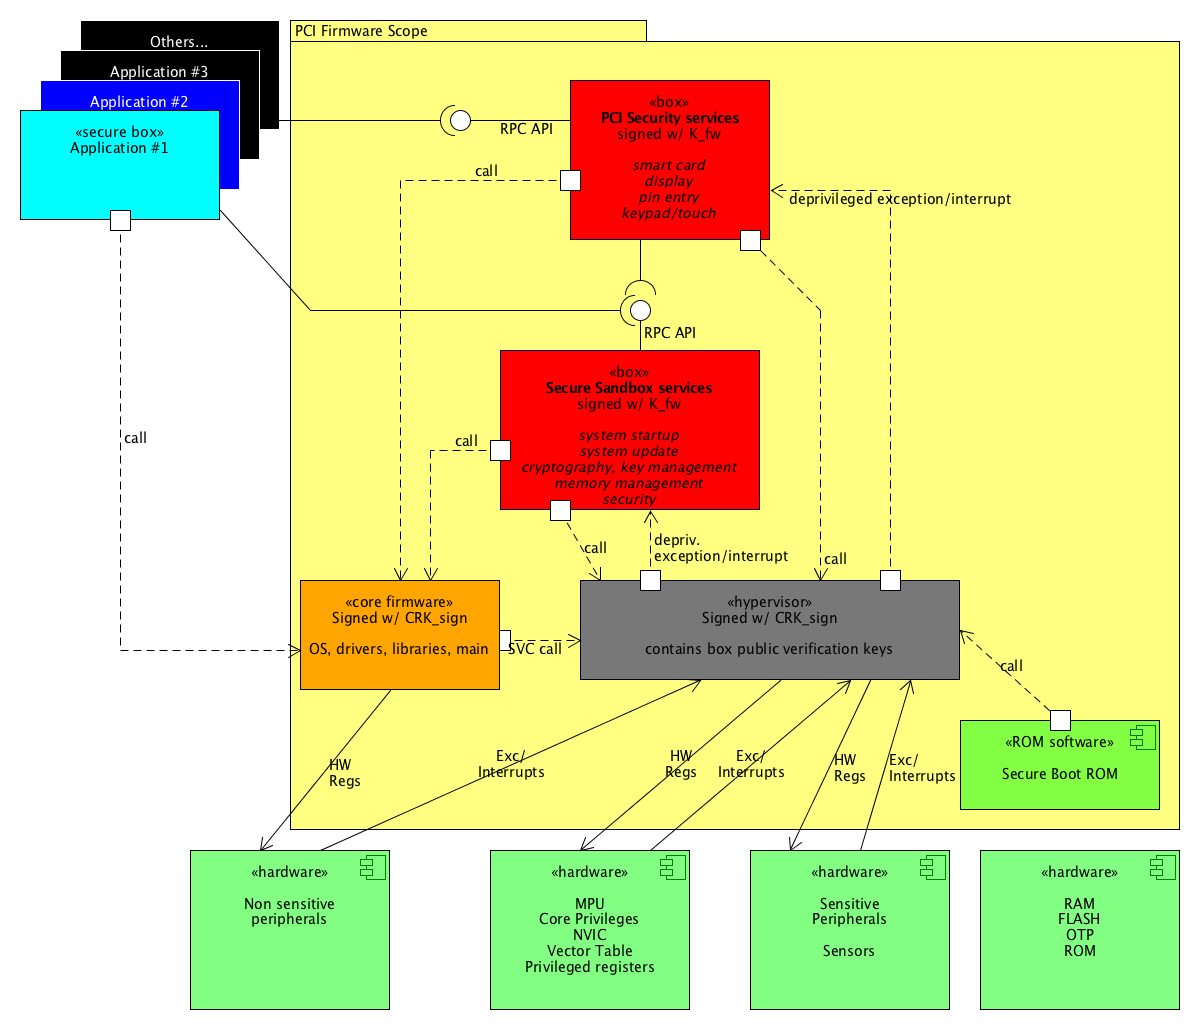
\includegraphics[width=\textwidth,height=\textheight/2,keepaspectratio=true]{pci_cortex.png}}
\end{DoxyImageNoCaption}
  

\hypertarget{group__os}{}\section{Operating system, drivers, C library, other libraries...}
\label{group__os}\index{Operating system, drivers, C library, other libraries...@{Operating system, drivers, C library, other libraries...}}
The following software items are not running in a separate box\+:


\begin{DoxyItemize}
\item operating system
\item libraries
\item device drivers
\end{DoxyItemize}

They are rather seen as common code that can be executed within the context of multiple boxes. Success or failure of the functions called depend on the context, i.\+e. the current A\+C\+Ls, as enforced by u\+Visor.

This group of software items is considered as firmware.

P\+R\+I\+V\+I\+L\+E\+GE L\+E\+V\+EL\+: Core Firmware 
\begin{DoxyImageNoCaption}
  \mbox{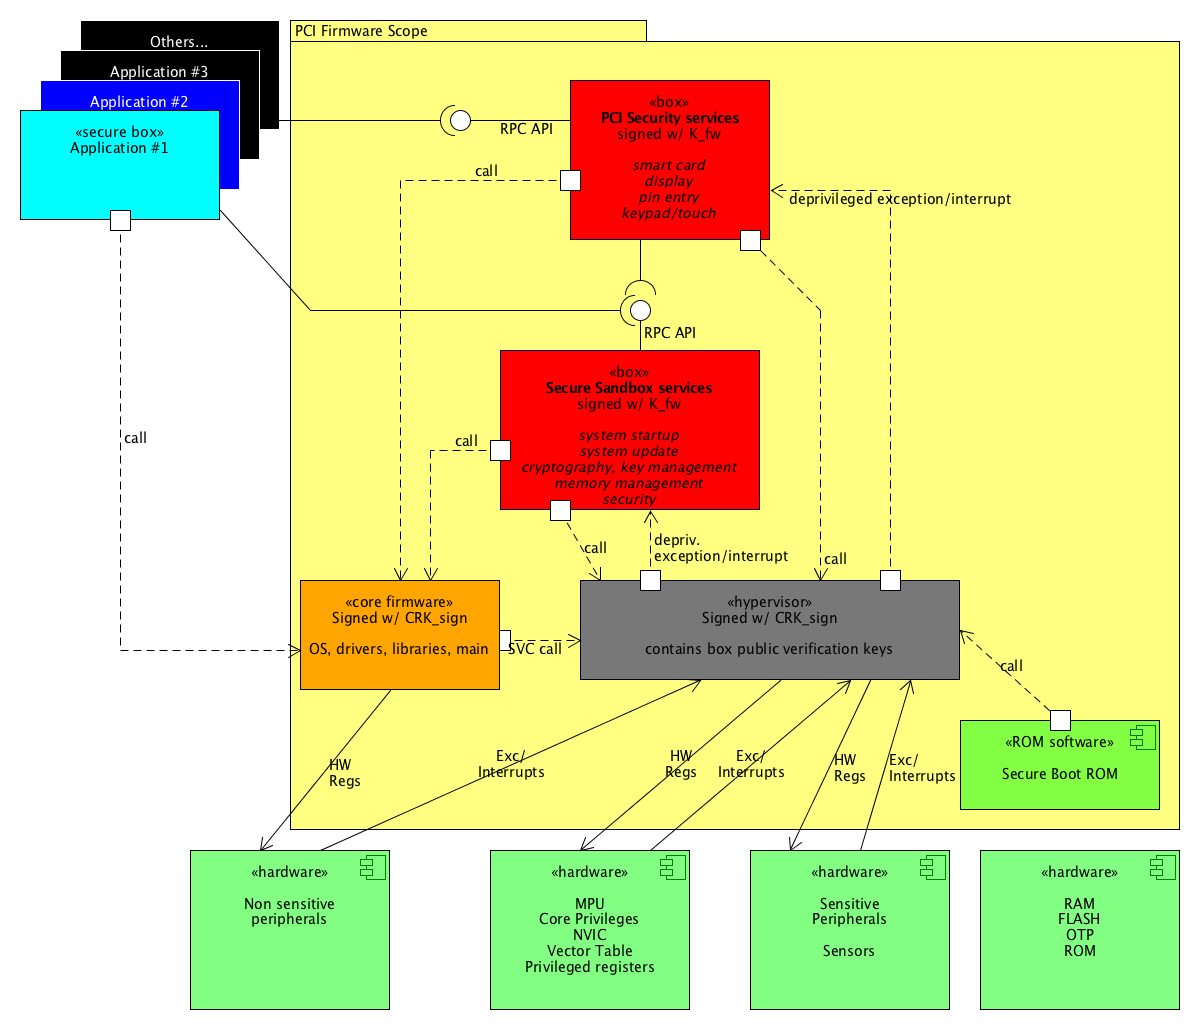
\includegraphics[width=\textwidth,height=\textheight/2,keepaspectratio=true]{pci_cortex.png}}
\end{DoxyImageNoCaption}
  

\hypertarget{group__smbx}{}\section{Security Monitor}
\label{group__smbx}\index{Security Monitor@{Security Monitor}}
This box is in charge of logging and handling security related events\+:
\begin{DoxyItemize}
\item non maskable interrupts due to security issues
\item uvisor related exceptions (access faults)
\end{DoxyItemize}

It allows other boxes to\+:
\begin{DoxyItemize}
\item register event handlers to different events
\item read the log
\end{DoxyItemize}

This box runs in an independent thread that\+:
\begin{DoxyItemize}
\item listens to R\+PC
\item responds to R\+PC calls and checks the privileges of the caller
\end{DoxyItemize}


\begin{DoxyImageNoCaption}
  \mbox{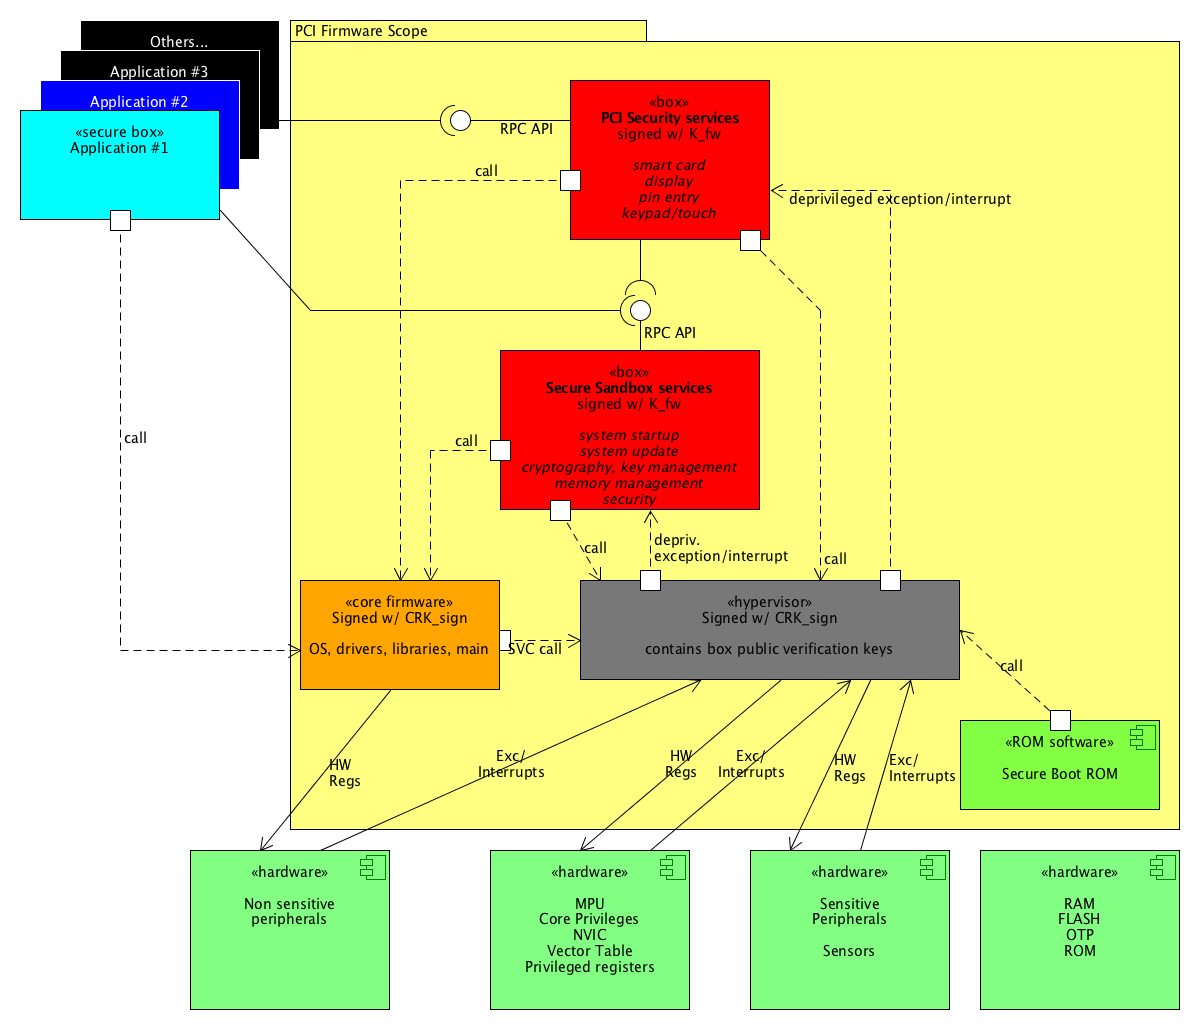
\includegraphics[width=\textwidth,height=\textheight/2,keepaspectratio=true]{pci_cortex.png}}
\end{DoxyImageNoCaption}
  

\hypertarget{group__ssbx}{}\section{Secure Sandbox services (Generic Security functions)}
\label{group__ssbx}\index{Secure Sandbox services (\+Generic Security functions)@{Secure Sandbox services (\+Generic Security functions)}}
\subsection*{Modules}
\begin{DoxyCompactItemize}
\item 
\hyperlink{group__ssbx___crypto}{Cryptography}
\item 
\hyperlink{group__ssbx___main}{Global management functions}
\item 
\hyperlink{group__ssbx___i_o}{I/\+O A\+PI}
\item 
\hyperlink{group__ssbx___key_management}{Key Manager}
\item 
\hyperlink{group__ssbx___mem}{Memory Manager}
\end{DoxyCompactItemize}


\subsection{Detailed Description}
The functions available here provide access to sensitive devices and services
\begin{DoxyItemize}
\item User I/O (touchscreen, keypad, display)
\item Cryptography services
\item Key manager
\item Data storage through memory manager
\item Global security management (including firmware update, system startup, response to attacks, integrity checks)
\item Register event handlers to different events, and read associated log
\begin{DoxyItemize}
\item non maskable interrupts due to security issues
\item uvisor related exceptions (access faults, rpc errors)
\end{DoxyItemize}
\item Periodic/one-\/shot alarm service
\end{DoxyItemize}

This box is the only box privileged to access some devices. Therefore it proposes various services to interact with those peripherals.

Associated services are accessed through R\+PC.

This box runs in an independent thread that\+:
\begin{DoxyItemize}
\item listens to R\+PC
\item responds to R\+PC calls and checks the privileges of the caller
\end{DoxyItemize}

P\+R\+I\+V\+I\+L\+E\+GE L\+E\+V\+EL\+: Box Firmware


\begin{DoxyImageNoCaption}
  \mbox{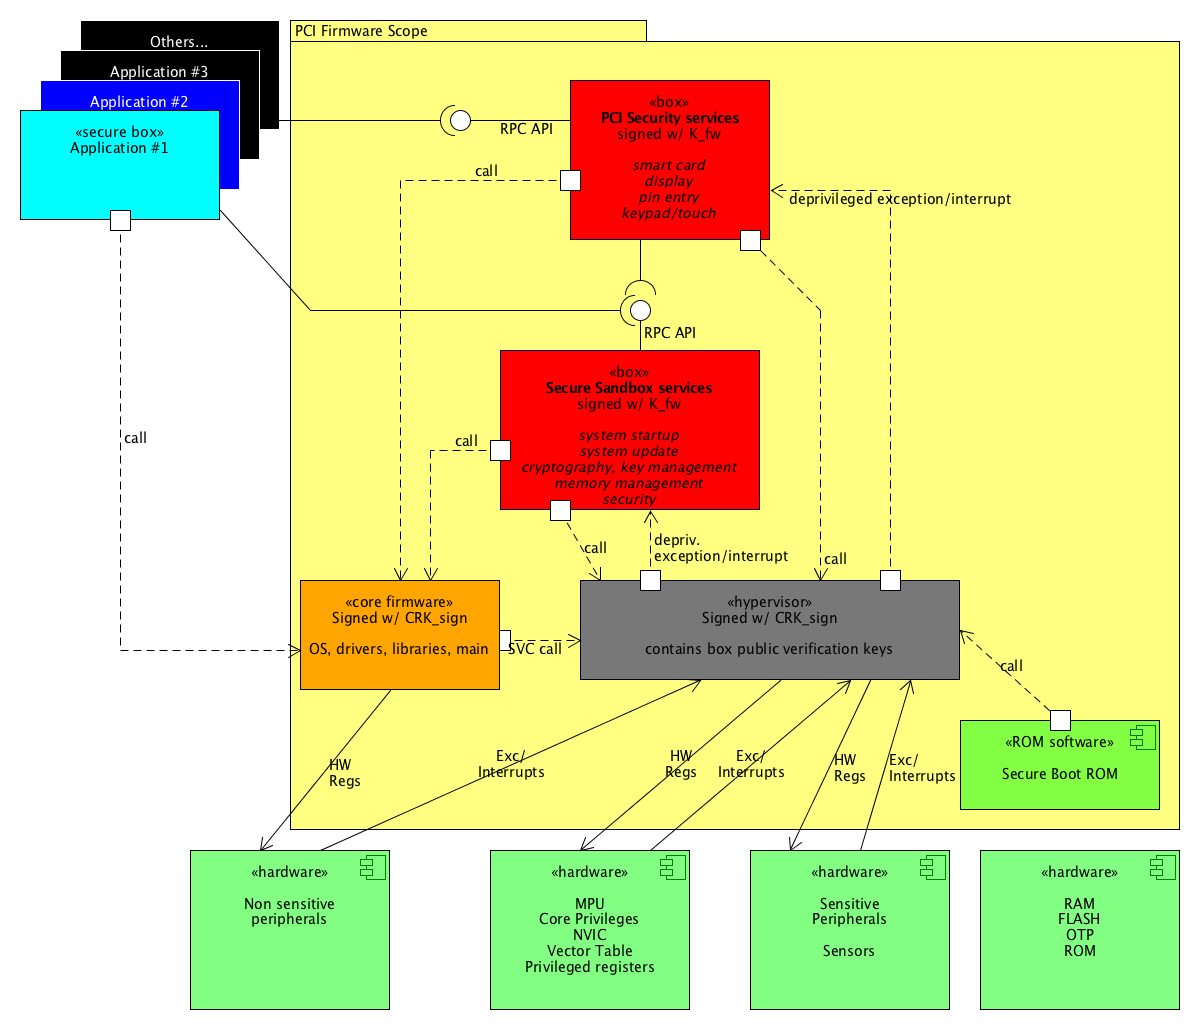
\includegraphics[width=\textwidth,height=\textheight/2,keepaspectratio=true]{pci_cortex.png}}
\end{DoxyImageNoCaption}
  
\shiftleveldown
\hypertarget{group__ssbx___crypto}{}\section{Cryptography}
\label{group__ssbx___crypto}\index{Cryptography@{Cryptography}}
This module offers a generic purpose cryptographic A\+PI.

The cryptographic A\+PI offers the following services\+:


\begin{DoxyItemize}
\item public key based signature/verification using R\+SA and E\+C\+D\+SA
\item symmetric encryption using 3\+D\+ES and A\+ES
\item message digest
\item M\+AC
\item D\+U\+K\+PT
\end{DoxyItemize}

It works in coordination with the Key Manager. 
\hypertarget{group__ssbx___main}{}\section{Global management functions}
\label{group__ssbx___main}\index{Global management functions@{Global management functions}}
Additional management services come from the u\+Visor A\+PI\+: \href{https://github.com/ARMmbed/uvisor/blob/master/docs/api/API.md}{\tt https\+://github.\+com/\+A\+R\+Mmbed/uvisor/blob/master/docs/api/\+A\+P\+I.\+md} 
\hypertarget{group__ssbx___i_o}{}\section{I/O A\+PI}
\label{group__ssbx___i_o}\index{I/\+O A\+PI@{I/\+O A\+PI}}
\subsection*{List of functions}
\begin{DoxyCompactItemize}
\item 
int \hyperlink{group__ssbx___i_o_ga52d5005d7bb36355592b9ef2309281e2}{ssbx\+\_\+display\+\_\+display\+\_\+image} (int image\+\_\+id)
\begin{DoxyCompactList}\small\item\em Displays a pre-\/defined image on the display. \end{DoxyCompactList}\item 
int \hyperlink{group__ssbx___i_o_ga701c4c43823bad80a39745de2b5ad3af}{ssbx\+\_\+display\+\_\+prompt} (unsigned char $\ast$kbd\+\_\+str, int $\ast$max\+\_\+length, int timeout, int message\+\_\+id, char mask, int font\+\_\+id)
\begin{DoxyCompactList}\small\item\em Displays a pre-\/defined prompt on the display and waits for user entry. \end{DoxyCompactList}\item 
int \hyperlink{group__ssbx___i_o_ga40574f625e50f59357a9c363305bf76e}{ssbx\+\_\+display\+\_\+write\+\_\+message} (int message\+\_\+id)
\begin{DoxyCompactList}\small\item\em Displays a pre-\/defined text message on the display. \end{DoxyCompactList}\item 
int \hyperlink{group__ssbx___i_o_gaefc88ab3af9c2f984281ac32723d0633}{ssbx\+\_\+touch\+\_\+get\+\_\+entry} (char $\ast$dest, int $\ast$len)
\begin{DoxyCompactList}\small\item\em Gets input from the virtual keypad on the touchscreen. \end{DoxyCompactList}\end{DoxyCompactItemize}


\subsection{Detailed Description}
This module offers some input-\/output services that allow interaction with users (keypad, touchscreen, display) 

\subsection{Function Documentation}
\hypertarget{group__ssbx___i_o_ga52d5005d7bb36355592b9ef2309281e2}{}\label{group__ssbx___i_o_ga52d5005d7bb36355592b9ef2309281e2} 
\index{I/\+O A\+PI@{I/\+O A\+PI}!ssbx\+\_\+display\+\_\+display\+\_\+image@{ssbx\+\_\+display\+\_\+display\+\_\+image}}
\index{ssbx\+\_\+display\+\_\+display\+\_\+image@{ssbx\+\_\+display\+\_\+display\+\_\+image}!I/\+O A\+PI@{I/\+O A\+PI}}
\subsubsection{\texorpdfstring{ssbx\+\_\+display\+\_\+display\+\_\+image()}{ssbx\_display\_display\_image()}}
{\footnotesize\ttfamily int ssbx\+\_\+display\+\_\+display\+\_\+image (\begin{DoxyParamCaption}\item[{int}]{image\+\_\+id }\end{DoxyParamCaption})}



Displays a pre-\/defined image on the display. 

Depending on the current state (see ssbx\+\_\+set\+\_\+state), the image will be displayed or an error will be returned.


\begin{DoxyParams}[1]{Parameters}
\mbox{\tt in}  & {\em image\+\_\+id} & The image identifier\\
\hline
\end{DoxyParams}
\begin{DoxyReturn}{Returns}
See error codes 
\end{DoxyReturn}
\hypertarget{group__ssbx___i_o_ga701c4c43823bad80a39745de2b5ad3af}{}\label{group__ssbx___i_o_ga701c4c43823bad80a39745de2b5ad3af} 
\index{I/\+O A\+PI@{I/\+O A\+PI}!ssbx\+\_\+display\+\_\+prompt@{ssbx\+\_\+display\+\_\+prompt}}
\index{ssbx\+\_\+display\+\_\+prompt@{ssbx\+\_\+display\+\_\+prompt}!I/\+O A\+PI@{I/\+O A\+PI}}
\subsubsection{\texorpdfstring{ssbx\+\_\+display\+\_\+prompt()}{ssbx\_display\_prompt()}}
{\footnotesize\ttfamily int ssbx\+\_\+display\+\_\+prompt (\begin{DoxyParamCaption}\item[{unsigned char $\ast$}]{kbd\+\_\+str,  }\item[{int $\ast$}]{max\+\_\+length,  }\item[{int}]{timeout,  }\item[{int}]{message\+\_\+id,  }\item[{char}]{mask,  }\item[{int}]{font\+\_\+id }\end{DoxyParamCaption})}



Displays a pre-\/defined prompt on the display and waits for user entry. 

Depending on the current state (see ssbx\+\_\+set\+\_\+state), the prompt will be displayed or an error will be returned.


\begin{DoxyParams}[1]{Parameters}
 & {\em kbd\+\_\+str} & The keyboard string \\
\hline
\mbox{\tt in}  & {\em timeout} & The timeout \\
\hline
\mbox{\tt in}  & {\em message\+\_\+id} & The message identifier \\
\hline
\mbox{\tt in}  & {\em mask} & The mask character to display in place of user input\\
\hline
\end{DoxyParams}
\begin{DoxyReturn}{Returns}
See error codes 
\end{DoxyReturn}
\hypertarget{group__ssbx___i_o_ga40574f625e50f59357a9c363305bf76e}{}\label{group__ssbx___i_o_ga40574f625e50f59357a9c363305bf76e} 
\index{I/\+O A\+PI@{I/\+O A\+PI}!ssbx\+\_\+display\+\_\+write\+\_\+message@{ssbx\+\_\+display\+\_\+write\+\_\+message}}
\index{ssbx\+\_\+display\+\_\+write\+\_\+message@{ssbx\+\_\+display\+\_\+write\+\_\+message}!I/\+O A\+PI@{I/\+O A\+PI}}
\subsubsection{\texorpdfstring{ssbx\+\_\+display\+\_\+write\+\_\+message()}{ssbx\_display\_write\_message()}}
{\footnotesize\ttfamily int ssbx\+\_\+display\+\_\+write\+\_\+message (\begin{DoxyParamCaption}\item[{int}]{message\+\_\+id }\end{DoxyParamCaption})}



Displays a pre-\/defined text message on the display. 

Depending on the current state (see ssbx\+\_\+set\+\_\+state), the text message will be displayed or an error will be returned.


\begin{DoxyParams}[1]{Parameters}
\mbox{\tt in}  & {\em message\+\_\+id} & The message identifier\\
\hline
\end{DoxyParams}
\begin{DoxyReturn}{Returns}
See error codes 
\end{DoxyReturn}
\hypertarget{group__ssbx___i_o_gaefc88ab3af9c2f984281ac32723d0633}{}\label{group__ssbx___i_o_gaefc88ab3af9c2f984281ac32723d0633} 
\index{I/\+O A\+PI@{I/\+O A\+PI}!ssbx\+\_\+touch\+\_\+get\+\_\+entry@{ssbx\+\_\+touch\+\_\+get\+\_\+entry}}
\index{ssbx\+\_\+touch\+\_\+get\+\_\+entry@{ssbx\+\_\+touch\+\_\+get\+\_\+entry}!I/\+O A\+PI@{I/\+O A\+PI}}
\subsubsection{\texorpdfstring{ssbx\+\_\+touch\+\_\+get\+\_\+entry()}{ssbx\_touch\_get\_entry()}}
{\footnotesize\ttfamily int ssbx\+\_\+touch\+\_\+get\+\_\+entry (\begin{DoxyParamCaption}\item[{char $\ast$}]{dest,  }\item[{int $\ast$}]{len }\end{DoxyParamCaption})}



Gets input from the virtual keypad on the touchscreen. 

This operation is allowed only if the P\+CI Secure Services box is not processing a P\+IN.


\begin{DoxyParams}[1]{Parameters}
 & {\em dest} & The destination \\
\hline
\mbox{\tt in,out}  & {\em len} & The key length\\
\hline
\end{DoxyParams}
\begin{DoxyReturn}{Returns}
See error codes 
\end{DoxyReturn}

\hypertarget{group__ssbx___key_management}{}\section{Key Manager}
\label{group__ssbx___key_management}\index{Key Manager@{Key Manager}}
The Key Manager allows secure importation, storage and execution of cryptographic keys in cryptographic protocols offered by the Cryptographic A\+PI. It also handles X.\+509 certificates (importation, verification, public key extraction).

Keys are assigned access rules that define what box can do what with the key (e.\+g. execute only, import, etc.) 
\hypertarget{group__ssbx___mem}{}\section{Memory Manager}
\label{group__ssbx___mem}\index{Memory Manager@{Memory Manager}}
This of module is in charge of securely handling the memory allocation/deallocation in N\+V\+S\+R\+AM. 
\restorelevel

\hypertarget{group__pcibx}{}\section{P\+CI Security Services, Security functions dedicated to P\+CI P\+TS P\+OI security}
\label{group__pcibx}\index{P\+C\+I Security Services, Security functions dedicated to P\+C\+I P\+T\+S P\+O\+I security@{P\+C\+I Security Services, Security functions dedicated to P\+C\+I P\+T\+S P\+O\+I security}}
\subsection*{Modules}
\begin{DoxyCompactItemize}
\item 
\hyperlink{group__pcibx__sc}{E\+M\+V-\/\+Level 1 Smart Card}
\item 
\hyperlink{group__pcibx___m_s_r}{Magnetic Stripe}
\item 
\hyperlink{group__pcibx___p_i_n}{P\+I\+N handling}
\end{DoxyCompactItemize}


\subsection{Detailed Description}
Security functions dedicated to P\+CI P\+TS P\+OI security are provided in this module, in particular for the P\+IN and Magnetic Stripe data handling, the Smart Card communication.

This box is the only box privileged to access some devices. Therefore it proposes various services to interact with those peripherals.

Associated services are accessed through R\+PC.

This box runs in an independent thread that\+:
\begin{DoxyItemize}
\item listens to R\+PC
\item responds to R\+PC calls and checks the privileges of the caller
\end{DoxyItemize}


\begin{DoxyImageNoCaption}
  \mbox{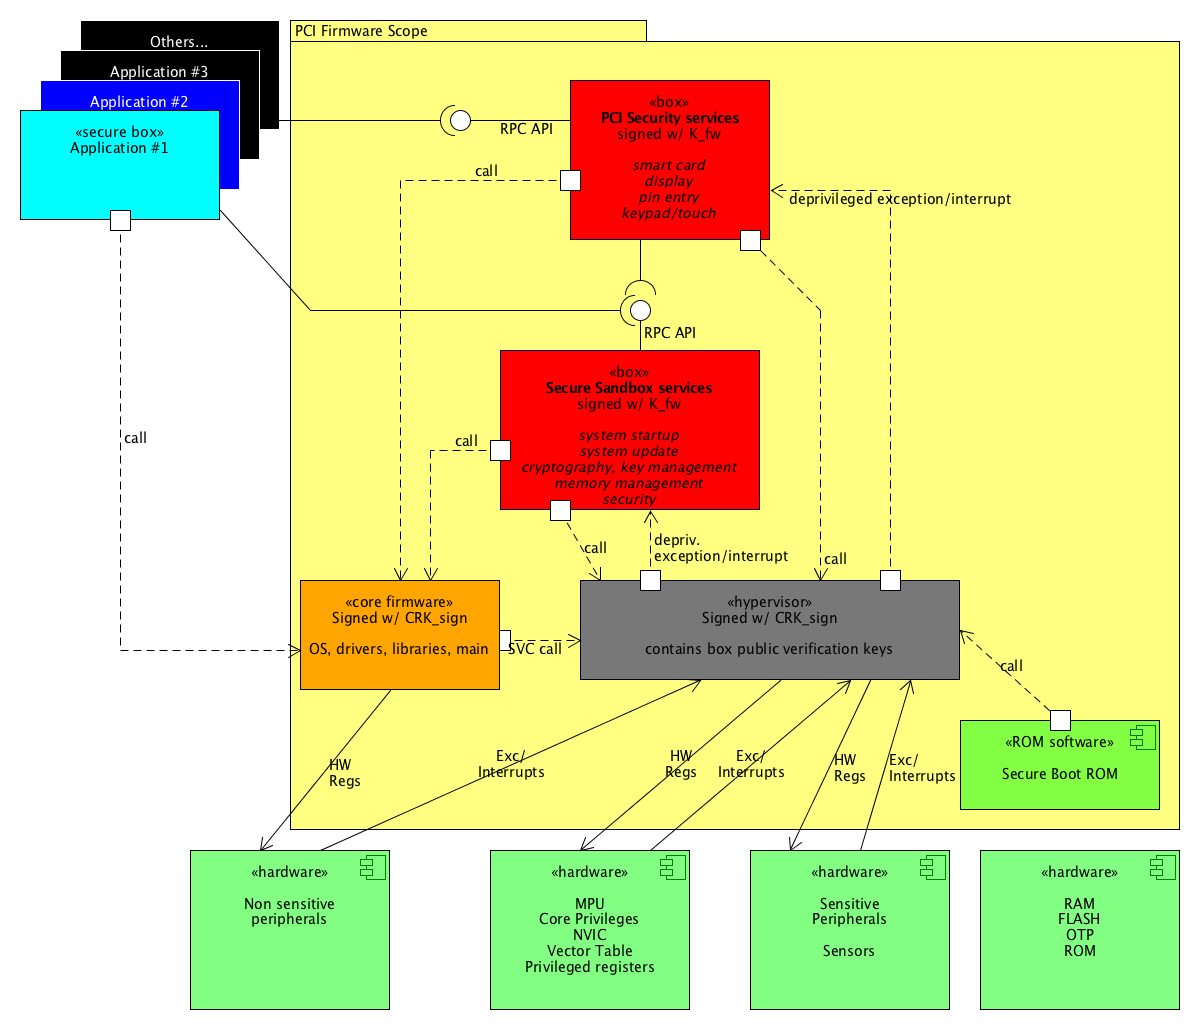
\includegraphics[width=\textwidth,height=\textheight/2,keepaspectratio=true]{pci_cortex.png}}
\end{DoxyImageNoCaption}
  
\shiftleveldown
\hypertarget{group__pcibx__sc}{}\section{E\+M\+V-\/\+Level 1 Smart Card}
\label{group__pcibx__sc}\index{E\+M\+V-\/\+Level 1 Smart Card@{E\+M\+V-\/\+Level 1 Smart Card}}
This of module is in charge of handling communication with Smart Cards while conforming to the E\+MV Level-\/1 specification. 
\hypertarget{group__pcibx___p_i_n}{}\section{P\+IN handling}
\label{group__pcibx___p_i_n}\index{P\+I\+N handling@{P\+I\+N handling}}
This module is in charge of handling P\+IN entry and processing according to the applicable P\+C\+T-\/\+P\+T\+S-\/\+P\+OI standard. 
\hypertarget{group__pcibx___m_s_r}{}\section{Magnetic Stripe}
\label{group__pcibx___m_s_r}\index{Magnetic Stripe@{Magnetic Stripe}}
P\+L\+A\+N\+N\+ED IN V2\+: This module is in charge of handling the magnetic stripe reading conforming to the S\+R\+ED requirements. 
\restorelevel


\hypertarget{group__hypervisor}{}\section{u\+Visor A\+PI}
\label{group__hypervisor}\index{u\+Visor A\+PI@{u\+Visor A\+PI}}
\subsection*{Data Structures}
\begin{DoxyCompactItemize}
\item 
struct \hyperlink{group__hypervisor_struct_uvisor_box_acl_item}{Uvisor\+Box\+Acl\+Item}
\end{DoxyCompactItemize}
\subsection*{Macros}
\begin{DoxyCompactItemize}
\item 
\#define \hyperlink{group__hypervisor_ga6143739a0475a71e8002f540de3c53f0}{U\+V\+I\+S\+O\+R\+\_\+\+B\+O\+X\+\_\+\+C\+O\+N\+F\+IG}(box\+\_\+nameconst Uv\+Box\+Acl\+Item module\+\_\+acl\+\_\+listuint32\+\_\+t module\+\_\+stack\+\_\+size,  struct \+\_\+\+\_\+your\+\_\+context,  verif\+\_\+key\+\_\+id)
\begin{DoxyCompactList}\small\item\em Secure box configuration. \end{DoxyCompactList}\item 
\#define \hyperlink{group__hypervisor_gafe52bfcc466d459d149c63966c2f4a58}{U\+V\+I\+S\+O\+R\+\_\+\+B\+O\+X\+\_\+\+N\+A\+M\+E\+S\+P\+A\+CE}(static const char const namespace)
\begin{DoxyCompactList}\small\item\em Specify the namespace for a box. C/\+C++ pre-\/processor macro (pseudo-\/function) \end{DoxyCompactList}\item 
\#define \hyperlink{group__hypervisor_ga7cb080278fc7d660addf9bbff6d3f2da}{U\+V\+I\+S\+O\+R\+\_\+\+S\+E\+T\+\_\+\+M\+O\+DE}(uvisor\+\_\+mode)
\begin{DoxyCompactList}\small\item\em Set mode for the u\+Visor \mbox{[}temporary\mbox{]}. \end{DoxyCompactList}\item 
\#define \hyperlink{group__hypervisor_gae90f548ce110da855610f79301aafe34}{U\+V\+I\+S\+O\+R\+\_\+\+S\+E\+T\+\_\+\+M\+O\+D\+E\+\_\+\+A\+CL}(uvisor\+\_\+mode,  const Uv\+Box\+Acl main\+\_\+box\+\_\+acl\+\_\+list)
\begin{DoxyCompactList}\small\item\em Set mode for the u\+Visor and provide background A\+C\+Ls for the main box. \end{DoxyCompactList}\end{DoxyCompactItemize}
\subsection*{List of types}
\begin{DoxyCompactItemize}
\item 
typedef uint32\+\_\+t \hyperlink{group__hypervisor_ga1527b3a7e3df3007490669cbd26b4fe9}{Uvisor\+Box\+Acl}
\end{DoxyCompactItemize}
\subsection*{List of functions}
\begin{DoxyCompactItemize}
\item 
int \hyperlink{group__hypervisor_ga6e7f7b03367daefa2cbcb7e4f0538ba7}{check\+\_\+acl} (uint32\+\_\+t $\ast$p\+\_\+acl, uint32\+\_\+t keyindex)
\begin{DoxyCompactList}\small\item\em Hook called by u\+Visor during loading of secure boxes. \end{DoxyCompactList}\item 
int \hyperlink{group__hypervisor_gafdaf52538986a558e934eab65221731e}{rpc\+\_\+fncall\+\_\+waitfor} (const T\+F\+N\+\_\+\+Ptr fn\+\_\+ptr\+\_\+array\mbox{[}$\,$\mbox{]}, size\+\_\+t fn\+\_\+count, int $\ast$box\+\_\+id\+\_\+caller, uint32\+\_\+t timeout\+\_\+ms)
\begin{DoxyCompactList}\small\item\em Handle incoming R\+PC, setting the parameter box\+\_\+id\+\_\+caller to the caller box ID. \end{DoxyCompactList}\item 
int \hyperlink{group__hypervisor_gab099ca7d08f626791039573dbff14af5}{uvisor\+\_\+box\+\_\+id\+\_\+self} (void)
\begin{DoxyCompactList}\small\item\em Get the ID of the current box. \end{DoxyCompactList}\item 
int \hyperlink{group__hypervisor_gab605e738e6bc828cd9efb6eacca79685}{uvisor\+\_\+box\+\_\+namespace} (int box\+\_\+id, char $\ast$box\+\_\+namespace, size\+\_\+t length)
\begin{DoxyCompactList}\small\item\em Copy the namespace of the specified box to the provided buffer. \end{DoxyCompactList}\item 
int \hyperlink{group__hypervisor_ga82e5cbff1a1a26974ed1e5f493607cf2}{uvisor\+\_\+box\+\_\+signingkey} (int box\+\_\+id, int $\ast$keyindex)
\begin{DoxyCompactList}\small\item\em Get the signing key ID of the specified box, hence its box privilege. \end{DoxyCompactList}\item 
void \hyperlink{group__hypervisor_gaa02ff863ab222f97723b60e59f6d92d8}{v\+I\+R\+Q\+\_\+\+Clear\+Pending\+I\+RQ} (uint32\+\_\+t irqn)
\begin{DoxyCompactList}\small\item\em Clear pending status of I\+R\+Qn. \end{DoxyCompactList}\item 
void \hyperlink{group__hypervisor_ga7beb8d1fe68378367bcb8085a2d16cd5}{v\+I\+R\+Q\+\_\+\+Disable\+I\+RQ} (uint32\+\_\+t irqn)
\begin{DoxyCompactList}\small\item\em Disable I\+R\+Qn for the currently active box. \end{DoxyCompactList}\item 
void \hyperlink{group__hypervisor_ga3dd01fda80a57db36a78994d0cae91ee}{v\+I\+R\+Q\+\_\+\+Enable\+I\+RQ} (uint32\+\_\+t irqn)
\begin{DoxyCompactList}\small\item\em Enable I\+R\+Qn for the currently active box. \end{DoxyCompactList}\item 
int \hyperlink{group__hypervisor_ga880e3229f62cfff1c638c5dd6a1e9050}{v\+I\+R\+Q\+\_\+\+Get\+Level} (void)
\begin{DoxyCompactList}\small\item\em Get level of currently active I\+R\+Qn, if any. \end{DoxyCompactList}\item 
uint32\+\_\+t \hyperlink{group__hypervisor_gad450b31ead2ec4f7bb2dbe07ebcfd8e7}{v\+I\+R\+Q\+\_\+\+Get\+Pending\+I\+RQ} (uint32\+\_\+t irqn)
\begin{DoxyCompactList}\small\item\em Get pending status of I\+R\+Qn. \end{DoxyCompactList}\item 
uint32\+\_\+t \hyperlink{group__hypervisor_ga3da0be917ac42157f0d33e3e1412379b}{v\+I\+R\+Q\+\_\+\+Get\+Priority} (uint32\+\_\+t irqn)
\begin{DoxyCompactList}\small\item\em Get priority level of I\+R\+Qn. \end{DoxyCompactList}\item 
uint32\+\_\+t \hyperlink{group__hypervisor_gaaa9c852e90077dd4c553240d769b3658}{v\+I\+R\+Q\+\_\+\+Get\+Vector} (uint32\+\_\+t irqn)
\begin{DoxyCompactList}\small\item\em Get the I\+SR registered for I\+R\+Qn. \end{DoxyCompactList}\item 
void \hyperlink{group__hypervisor_gab5570c2fa5a04a3a183cdef960a43c6b}{v\+I\+R\+Q\+\_\+\+Set\+Pending\+I\+RQ} (uint32\+\_\+t irqn)
\begin{DoxyCompactList}\small\item\em Set pending status of I\+R\+Qn. \end{DoxyCompactList}\item 
void \hyperlink{group__hypervisor_ga3c725e15df2f30fdaed9f1873a7eebdf}{v\+I\+R\+Q\+\_\+\+Set\+Priority} (uint32\+\_\+t irqn, uint32\+\_\+t priority)
\begin{DoxyCompactList}\small\item\em Set priority level of I\+R\+Qn. \end{DoxyCompactList}\item 
void \hyperlink{group__hypervisor_ga3bf7917bc9150d1b91bec5d41962ff13}{v\+I\+R\+Q\+\_\+\+Set\+Vector} (uint32\+\_\+t irqn, uint32\+\_\+t vector)
\begin{DoxyCompactList}\small\item\em Register an I\+SR to the currently active box. \end{DoxyCompactList}\end{DoxyCompactItemize}


\subsection{Detailed Description}
The payment application is to be developed by the payment terminal vendor. It dialogs with the 2 secure boxes through remote procedure calls (R\+PC). The A\+PI is described below in this document. Shortly this A\+PI allows to display trusted messages on the display, perform E\+M\+V-\/level 1 compliant A\+P\+DU exchanges with the smart card, perform P\+IN processing, capture Mag Stripe… basically everything required to perform an E\+MV Level-\/2 compliant payment.

Here you can find detailed documentation for\+:


\begin{DoxyEnumerate}
\item \href{#configuration-macros}{\tt Configuration macros}, to configure a secure box and protect data and peripherals.
\item \href{#box-identity}{\tt Box Identity}, to retrieve a box-\/specific ID or the namespace of the current or calling box.
\begin{DoxyItemize}
\item A box identity identifies a security domain uniquely and globally.
\item The box identity A\+PI can be used to determine the source box of an inbound secure gateway call. This can be useful for implementing complex authorization logic between mutually distrustful security domains.
\item u\+Visor provides the ability to retrieve the box ID of the current box ({\ttfamily uvisor\+\_\+box\+\_\+id\+\_\+self}), or of the box that called the current box through an R\+PC gateway via the {\ttfamily box\+\_\+id\+\_\+caller} parameter of {\ttfamily rpc\+\_\+fncall\+\_\+waitfor}.
\item The box ID number is not constant and can change between reboots. But, the box ID number can be used as a token to retrieve a constant string identifier, known as the box namespace.
\item A box namespace is a static, box-\/specific string, that can help identify which box has which ID at run-\/time. In the future, the box namespace will be guaranteed to be globally unique.
\item A full example using this A\+PI is available at \href{https://github.com/ARMmbed/mbed-os-example-uvisor-number-store}{\tt mbed-\/os-\/example-\/uvisor-\/number-\/store}.
\end{DoxyItemize}
\item \href{#low-level-apis}{\tt Low level A\+P\+Is}, to access u\+Visor functions that are not available to unprivileged code (interrupts, restricted system registers).
\item \href{#type-definitions}{\tt Type definitions}.
\item \href{#error-codes}{\tt Error codes}.
\end{DoxyEnumerate}

\tabulinesep=1mm
\begin{longtabu} spread 0pt [c]{*{2}{|X[-1]}|}
\hline
\rowcolor{\tableheadbgcolor}{\bf Error reason }&{\bf Error code  }\\\cline{1-2}
\endfirsthead
\hline
\endfoot
\hline
\rowcolor{\tableheadbgcolor}{\bf Error reason }&{\bf Error code  }\\\cline{1-2}
\endhead
{\ttfamily P\+E\+R\+M\+I\+S\+S\+I\+O\+N\+\_\+\+D\+E\+N\+I\+ED} &1 \\\cline{1-2}
{\ttfamily S\+A\+N\+I\+T\+Y\+\_\+\+C\+H\+E\+C\+K\+\_\+\+F\+A\+I\+L\+ED} &2 \\\cline{1-2}
{\ttfamily N\+O\+T\+\_\+\+I\+M\+P\+L\+E\+M\+E\+N\+T\+ED} &3 \\\cline{1-2}
{\ttfamily N\+O\+T\+\_\+\+A\+L\+L\+O\+W\+ED} &4 \\\cline{1-2}
{\ttfamily F\+A\+U\+L\+T\+\_\+\+M\+E\+M\+M\+A\+N\+A\+GE} &5 \\\cline{1-2}
{\ttfamily F\+A\+U\+L\+T\+\_\+\+B\+US} &6 \\\cline{1-2}
{\ttfamily F\+A\+U\+L\+T\+\_\+\+U\+S\+A\+GE} &7 \\\cline{1-2}
{\ttfamily F\+A\+U\+L\+T\+\_\+\+H\+A\+RD} &8 \\\cline{1-2}
{\ttfamily F\+A\+U\+L\+T\+\_\+\+D\+E\+B\+UG} &9 \\\cline{1-2}
\end{longtabu}


\subsection{Data Structure Documentation}
\index{Uvisor\+Box\+Acl\+Item@{Uvisor\+Box\+Acl\+Item}}\label{struct_uvisor_box_acl_item}
\hypertarget{group__hypervisor_struct_uvisor_box_acl_item}{}
\subsubsection{struct Uvisor\+Box\+Acl\+Item}
\{ item\+\_\+description \} \begin{DoxyFields}{Data Fields}
\hypertarget{group__hypervisor_ae5e1b8a311ba7d63a3380828d266bc82}{}\label{group__hypervisor_ae5e1b8a311ba7d63a3380828d266bc82} 
\hyperlink{group__hypervisor_ga1527b3a7e3df3007490669cbd26b4fe9}{Uvisor\+Box\+Acl}&
acl&
\\
\hline

\hypertarget{group__hypervisor_aebb70c2aab3407a9f05334c47131a43b}{}\label{group__hypervisor_aebb70c2aab3407a9f05334c47131a43b} 
uint32\+\_\+t&
length&
\\
\hline

\hypertarget{group__hypervisor_a8cb9377ef5ed00f632f5744aa51f7b81}{}\label{group__hypervisor_a8cb9377ef5ed00f632f5744aa51f7b81} 
const volatile void $\ast$&
start&
\\
\hline

\end{DoxyFields}


\subsection{Macro Definition Documentation}
\hypertarget{group__hypervisor_ga6143739a0475a71e8002f540de3c53f0}{}\label{group__hypervisor_ga6143739a0475a71e8002f540de3c53f0} 
\index{u\+Visor A\+PI@{u\+Visor A\+PI}!U\+V\+I\+S\+O\+R\+\_\+\+B\+O\+X\+\_\+\+C\+O\+N\+F\+IG@{U\+V\+I\+S\+O\+R\+\_\+\+B\+O\+X\+\_\+\+C\+O\+N\+F\+IG}}
\index{U\+V\+I\+S\+O\+R\+\_\+\+B\+O\+X\+\_\+\+C\+O\+N\+F\+IG@{U\+V\+I\+S\+O\+R\+\_\+\+B\+O\+X\+\_\+\+C\+O\+N\+F\+IG}!u\+Visor A\+PI@{u\+Visor A\+PI}}
\subsubsection{\texorpdfstring{U\+V\+I\+S\+O\+R\+\_\+\+B\+O\+X\+\_\+\+C\+O\+N\+F\+IG}{UVISOR\_BOX\_CONFIG}}
{\footnotesize\ttfamily \#define U\+V\+I\+S\+O\+R\+\_\+\+B\+O\+X\+\_\+\+C\+O\+N\+F\+IG(\begin{DoxyParamCaption}\item[{}]{box\+\_\+nameconst Uv\+Box\+Acl\+Item module\+\_\+acl\+\_\+listuint32\+\_\+tmodule\+\_\+stack\+\_\+size,  }\item[{}]{struct \+\_\+\+\_\+your\+\_\+context,  }\item[{}]{verif\+\_\+key\+\_\+id }\end{DoxyParamCaption})}



Secure box configuration. 

C/\+C++ pre-\/processor macro (pseudo-\/function)


\begin{DoxyParams}{Parameters}
{\em box\+\_\+name} & Secure box name \\
\hline
{\em module\+\_\+acl\+\_\+list} & List of A\+C\+Ls for the module \\
\hline
{\em module\+\_\+stack\+\_\+size} & Required stack size for the secure box \\
\hline
{\em \+\_\+\+\_\+your\+\_\+context} & \mbox{[}optional\mbox{]} Type definition of the struct hosting the box context data \\
\hline
{\em verif\+\_\+key\+\_\+id} & the Id of the key to use for the verification of the signature of the box \#define K\+E\+Y\+I\+N\+D\+E\+X\+\_\+\+FW 0x4\+E5\+F739a\+UL \#define K\+E\+Y\+I\+N\+D\+E\+X\+\_\+\+T\+R\+U\+S\+T\+E\+D\+A\+PP 0xebf78ac4\+UL \#define K\+E\+Y\+I\+N\+D\+E\+X\+\_\+\+O\+T\+H\+E\+R\+A\+PP 0x9cfb3459\+UL\\
\hline
\end{DoxyParams}
Example\+: ``` \#include \char`\"{}uvisor-\/lib/uvisor-\/lib.\+h\char`\"{}

// Required stack size \#define B\+O\+X\+\_\+\+S\+T\+A\+C\+K\+\_\+\+S\+I\+ZE 0x100

// Define the box context. typedef struct \{ uint8\+\_\+t secret\mbox{[}S\+E\+C\+R\+E\+T\+\_\+\+S\+I\+ZE\mbox{]}; bool initialized; State\+\_\+t current\+\_\+state \} Box\+Context;

// Create the A\+CL list for the module. static const Uv\+Box\+Acl\+Item g\+\_\+box\+\_\+acl\mbox{[}\mbox{]} = \{ \{P\+O\+R\+TB, sizeof($\ast$\+P\+O\+R\+T\+B), U\+V\+I\+S\+O\+R\+\_\+\+T\+A\+C\+L\+D\+E\+F\+\_\+\+P\+E\+R\+I\+PH\}, \{R\+TC, sizeof($\ast$\+R\+T\+C), $\ast$ U\+V\+I\+S\+O\+R\+\_\+\+T\+A\+C\+L\+D\+E\+F\+\_\+\+P\+E\+R\+I\+PH\}, \{L\+P\+T\+M\+R0, sizeof($\ast$\+L\+P\+T\+M\+R0), U\+V\+I\+S\+O\+R\+\_\+\+T\+A\+C\+L\+D\+E\+F\+\_\+\+P\+E\+R\+I\+PH\}, \};

// Configure the secure box compartment. U\+V\+I\+S\+O\+R\+\_\+\+B\+O\+X\+\_\+\+N\+A\+M\+E\+S\+P\+A\+CE(\char`\"{}com.\+example.\+my-\/box-\/name\char`\"{}); U\+V\+I\+S\+O\+R\+\_\+\+B\+O\+X\+\_\+\+C\+O\+N\+F\+IG(my\+\_\+box\+\_\+name, g\+\_\+box\+\_\+acl, B\+O\+X\+\_\+\+S\+T\+A\+C\+K\+\_\+\+S\+I\+ZE, Box\+Context);

``` \hypertarget{group__hypervisor_gafe52bfcc466d459d149c63966c2f4a58}{}\label{group__hypervisor_gafe52bfcc466d459d149c63966c2f4a58} 
\index{u\+Visor A\+PI@{u\+Visor A\+PI}!U\+V\+I\+S\+O\+R\+\_\+\+B\+O\+X\+\_\+\+N\+A\+M\+E\+S\+P\+A\+CE@{U\+V\+I\+S\+O\+R\+\_\+\+B\+O\+X\+\_\+\+N\+A\+M\+E\+S\+P\+A\+CE}}
\index{U\+V\+I\+S\+O\+R\+\_\+\+B\+O\+X\+\_\+\+N\+A\+M\+E\+S\+P\+A\+CE@{U\+V\+I\+S\+O\+R\+\_\+\+B\+O\+X\+\_\+\+N\+A\+M\+E\+S\+P\+A\+CE}!u\+Visor A\+PI@{u\+Visor A\+PI}}
\subsubsection{\texorpdfstring{U\+V\+I\+S\+O\+R\+\_\+\+B\+O\+X\+\_\+\+N\+A\+M\+E\+S\+P\+A\+CE}{UVISOR\_BOX\_NAMESPACE}}
{\footnotesize\ttfamily \#define U\+V\+I\+S\+O\+R\+\_\+\+B\+O\+X\+\_\+\+N\+A\+M\+E\+S\+P\+A\+CE(\begin{DoxyParamCaption}\item[{}]{static const char constnamespace }\end{DoxyParamCaption})}



Specify the namespace for a box. C/\+C++ pre-\/processor macro (pseudo-\/function) 


\begin{DoxyParams}{Parameters}
{\em namespace} & The namespace of the box\\
\hline
\end{DoxyParams}
The namespace of the box must be a null-\/terminated string no longer than M\+A\+X\+\_\+\+B\+O\+X\+\_\+\+N\+A\+M\+E\+S\+P\+A\+C\+E\+\_\+\+L\+E\+N\+G\+TH (including the terminating null).

The namespace must also be stored in public flash. u\+Visor will verify that the namespace is null-\/terminated and stored in public flash at boot-\/time, and will halt if the namespace fails this verification. For now, use a reverse domain name for the box namespace.

If you don\textquotesingle{}t have a reverse domain name, use a G\+U\+ID string identifier. We currently don\textquotesingle{}t verify that the namespace is globally unique, but we will perform this validation in the future.

Use of this configuration macro before U\+V\+I\+S\+O\+R\+\_\+\+B\+O\+X\+\_\+\+C\+O\+N\+F\+IG is required. If you do not wish to give your box a namespace, specify N\+U\+LL as the namespace to create an anonymous box.

Example\+: 
\begin{DoxyCode}
\textcolor{preprocessor}{#include "uvisor-lib/uvisor-lib.h"}

\textcolor{comment}{// Configure the secure box.}
\hyperlink{group__hypervisor_gafe52bfcc466d459d149c63966c2f4a58}{UVISOR\_BOX\_NAMESPACE}(\textcolor{stringliteral}{"com.example.my-box-name"});
\hyperlink{group__hypervisor_ga6143739a0475a71e8002f540de3c53f0}{UVISOR\_BOX\_CONFIG}(my\_box\_name, UVISOR\_BOX\_STACK\_SIZE); 
\end{DoxyCode}
 \hypertarget{group__hypervisor_ga7cb080278fc7d660addf9bbff6d3f2da}{}\label{group__hypervisor_ga7cb080278fc7d660addf9bbff6d3f2da} 
\index{u\+Visor A\+PI@{u\+Visor A\+PI}!U\+V\+I\+S\+O\+R\+\_\+\+S\+E\+T\+\_\+\+M\+O\+DE@{U\+V\+I\+S\+O\+R\+\_\+\+S\+E\+T\+\_\+\+M\+O\+DE}}
\index{U\+V\+I\+S\+O\+R\+\_\+\+S\+E\+T\+\_\+\+M\+O\+DE@{U\+V\+I\+S\+O\+R\+\_\+\+S\+E\+T\+\_\+\+M\+O\+DE}!u\+Visor A\+PI@{u\+Visor A\+PI}}
\subsubsection{\texorpdfstring{U\+V\+I\+S\+O\+R\+\_\+\+S\+E\+T\+\_\+\+M\+O\+DE}{UVISOR\_SET\_MODE}}
{\footnotesize\ttfamily \#define U\+V\+I\+S\+O\+R\+\_\+\+S\+E\+T\+\_\+\+M\+O\+DE(\begin{DoxyParamCaption}\item[{}]{uvisor\+\_\+mode }\end{DoxyParamCaption})}



Set mode for the u\+Visor \mbox{[}temporary\mbox{]}. 

C/\+C++ pre-\/processor macro (object declaration)


\begin{DoxyParams}[1]{Parameters}
\mbox{\tt in}  & {\em uvisor\+\_\+mode} & The uvisor mode\+:
\begin{DoxyItemize}
\item U\+V\+I\+S\+O\+R\+\_\+\+D\+I\+S\+A\+B\+L\+ED = disabled \mbox{[}default\mbox{]}
\item U\+V\+I\+S\+O\+R\+\_\+\+P\+E\+R\+M\+I\+S\+S\+I\+VE = permissive \mbox{[}currently n.\+a.\mbox{]}
\item U\+V\+I\+S\+O\+R\+\_\+\+E\+N\+A\+B\+L\+ED = enabled
\end{DoxyItemize}\\
\hline
\end{DoxyParams}
Example\+:


\begin{DoxyCode}
\textcolor{preprocessor}{#include "uvisor-lib/uvisor-lib.h"}

\textcolor{comment}{// Set the uVisor mode. }
\hyperlink{group__hypervisor_ga7cb080278fc7d660addf9bbff6d3f2da}{UVISOR\_SET\_MODE}(UVISOR\_ENABLED);
\end{DoxyCode}


{\bfseries Note\+:}


\begin{DoxyEnumerate}
\item This macro is only needed temporarily (u\+Visor disabled by default) and will be removed in the future.
\item This macro must be used only once in the top level yotta executable. 
\end{DoxyEnumerate}\hypertarget{group__hypervisor_gae90f548ce110da855610f79301aafe34}{}\label{group__hypervisor_gae90f548ce110da855610f79301aafe34} 
\index{u\+Visor A\+PI@{u\+Visor A\+PI}!U\+V\+I\+S\+O\+R\+\_\+\+S\+E\+T\+\_\+\+M\+O\+D\+E\+\_\+\+A\+CL@{U\+V\+I\+S\+O\+R\+\_\+\+S\+E\+T\+\_\+\+M\+O\+D\+E\+\_\+\+A\+CL}}
\index{U\+V\+I\+S\+O\+R\+\_\+\+S\+E\+T\+\_\+\+M\+O\+D\+E\+\_\+\+A\+CL@{U\+V\+I\+S\+O\+R\+\_\+\+S\+E\+T\+\_\+\+M\+O\+D\+E\+\_\+\+A\+CL}!u\+Visor A\+PI@{u\+Visor A\+PI}}
\subsubsection{\texorpdfstring{U\+V\+I\+S\+O\+R\+\_\+\+S\+E\+T\+\_\+\+M\+O\+D\+E\+\_\+\+A\+CL}{UVISOR\_SET\_MODE\_ACL}}
{\footnotesize\ttfamily \#define U\+V\+I\+S\+O\+R\+\_\+\+S\+E\+T\+\_\+\+M\+O\+D\+E\+\_\+\+A\+CL(\begin{DoxyParamCaption}\item[{}]{uvisor\+\_\+mode,  }\item[{}]{const Uv\+Box\+Aclmain\+\_\+box\+\_\+acl\+\_\+list }\end{DoxyParamCaption})}



Set mode for the u\+Visor and provide background A\+C\+Ls for the main box. 

C/\+C++ pre-\/processor macro (object declaration)


\begin{DoxyParams}[1]{Parameters}
\mbox{\tt in}  & {\em uvisor\+\_\+mode} & The uvisor mode
\begin{DoxyItemize}
\item U\+V\+I\+S\+O\+R\+\_\+\+D\+I\+S\+A\+B\+L\+ED$<$ = disabled \mbox{[}default\mbox{]}
\item U\+V\+I\+S\+O\+R\+\_\+\+P\+E\+R\+M\+I\+S\+S\+I\+VE = permissive \mbox{[}currently n.\+a.\mbox{]}
\item U\+V\+I\+S\+O\+R\+\_\+\+E\+N\+A\+B\+L\+ED = enabled
\end{DoxyItemize}\\
\hline
 & {\em main\+\_\+box\+\_\+acl\+\_\+list} & List of A\+C\+Ls for the main box (background A\+C\+Ls)\\
\hline
\end{DoxyParams}
Example\+:


\begin{DoxyCode}
\textcolor{preprocessor}{#include "uvisor-lib/uvisor-lib.h"}
\textcolor{comment}{// Create background ACLs for the main box. }
\textcolor{keyword}{static} \textcolor{keyword}{const} UvBoxAclItem g\_background\_acl[] = \{
  \{UART0,       \textcolor{keyword}{sizeof}(*UART0), UVISOR\_TACL\_PERIPHERAL\},
  \{UART1,       \textcolor{keyword}{sizeof}(*UART1), UVISOR\_TACL\_PERIPHERAL\},
  \{PIT,         \textcolor{keyword}{sizeof}(*PIT),   UVISOR\_TACL\_PERIPHERAL\},
\};

\textcolor{comment}{// Set the uVisor mode. }
\hyperlink{group__hypervisor_gae90f548ce110da855610f79301aafe34}{UVISOR\_SET\_MODE\_ACL}(UVISOR\_ENABLED, g\_background\_acl);
\end{DoxyCode}


{\bfseries Note\+:}


\begin{DoxyEnumerate}
\item This macro is only needed temporarily (u\+Visor disabled by default) and will be removed in the future.
\item This macro must be used only once in the top level yotta executable. 
\end{DoxyEnumerate}

\subsection{Typedef Documentation}
\hypertarget{group__hypervisor_ga1527b3a7e3df3007490669cbd26b4fe9}{}\label{group__hypervisor_ga1527b3a7e3df3007490669cbd26b4fe9} 
\index{u\+Visor A\+PI@{u\+Visor A\+PI}!Uvisor\+Box\+Acl@{Uvisor\+Box\+Acl}}
\index{Uvisor\+Box\+Acl@{Uvisor\+Box\+Acl}!u\+Visor A\+PI@{u\+Visor A\+PI}}
\subsubsection{\texorpdfstring{Uvisor\+Box\+Acl}{UvisorBoxAcl}}
{\footnotesize\ttfamily typedef uint32\+\_\+t \hyperlink{group__hypervisor_ga1527b3a7e3df3007490669cbd26b4fe9}{Uvisor\+Box\+Acl}}

\{ item\+\_\+description \} 

\subsection{Function Documentation}
\hypertarget{group__hypervisor_ga6e7f7b03367daefa2cbcb7e4f0538ba7}{}\label{group__hypervisor_ga6e7f7b03367daefa2cbcb7e4f0538ba7} 
\index{u\+Visor A\+PI@{u\+Visor A\+PI}!check\+\_\+acl@{check\+\_\+acl}}
\index{check\+\_\+acl@{check\+\_\+acl}!u\+Visor A\+PI@{u\+Visor A\+PI}}
\subsubsection{\texorpdfstring{check\+\_\+acl()}{check\_acl()}}
{\footnotesize\ttfamily int check\+\_\+acl (\begin{DoxyParamCaption}\item[{uint32\+\_\+t $\ast$}]{p\+\_\+acl,  }\item[{uint32\+\_\+t}]{keyindex }\end{DoxyParamCaption})}



Hook called by u\+Visor during loading of secure boxes. 

It is the responsibility of the platform developer to implement this function to restrict A\+C\+Ls based on the box privilege of the box being loaded.


\begin{DoxyParams}[1]{Parameters}
 & {\em p\+\_\+acl} & Pointer to the A\+CL of the box being loaded \\
\hline
\mbox{\tt in}  & {\em keyindex} & The key used to verify the box (hence its box privilege)\\
\hline
\end{DoxyParams}
\begin{DoxyReturn}{Returns}
0 if the A\+CL conforms to the A\+CL policy 
\end{DoxyReturn}
\hypertarget{group__hypervisor_gafdaf52538986a558e934eab65221731e}{}\label{group__hypervisor_gafdaf52538986a558e934eab65221731e} 
\index{u\+Visor A\+PI@{u\+Visor A\+PI}!rpc\+\_\+fncall\+\_\+waitfor@{rpc\+\_\+fncall\+\_\+waitfor}}
\index{rpc\+\_\+fncall\+\_\+waitfor@{rpc\+\_\+fncall\+\_\+waitfor}!u\+Visor A\+PI@{u\+Visor A\+PI}}
\subsubsection{\texorpdfstring{rpc\+\_\+fncall\+\_\+waitfor()}{rpc\_fncall\_waitfor()}}
{\footnotesize\ttfamily int rpc\+\_\+fncall\+\_\+waitfor (\begin{DoxyParamCaption}\item[{const T\+F\+N\+\_\+\+Ptr}]{fn\+\_\+ptr\+\_\+array\mbox{[}$\,$\mbox{]},  }\item[{size\+\_\+t}]{fn\+\_\+count,  }\item[{int $\ast$}]{box\+\_\+id\+\_\+caller,  }\item[{uint32\+\_\+t}]{timeout\+\_\+ms }\end{DoxyParamCaption})}



Handle incoming R\+PC, setting the parameter box\+\_\+id\+\_\+caller to the caller box ID. 

When deciding which memory to provide for rpc\+\_\+fncall\+\_\+waitfor to use when writing {\ttfamily box\+\_\+id\+\_\+caller}, strongly prefer thread local storage when multiple threads in a box can handle incoming R\+PC.


\begin{DoxyParams}[1]{Parameters}
\mbox{\tt in}  & {\em fn\+\_\+ptr\+\_\+array} & The function pointer array \\
\hline
\mbox{\tt in}  & {\em fn\+\_\+count} & The function count \\
\hline
 & {\em box\+\_\+id\+\_\+caller} & The box identifier of the caller. After a call, box\+\_\+id\+\_\+caller is set to the box ID of the calling box (the source box of the R\+PC). This is set before the R\+PC is dispatched, so that the R\+PC target function can read from this location to determine the calling box ID. This parameter is optional. \\
\hline
\mbox{\tt in}  & {\em timeout\+\_\+ms} & The timeout milliseconds\\
\hline
\end{DoxyParams}
\begin{DoxyReturn}{Returns}
\{ description\+\_\+of\+\_\+the\+\_\+return\+\_\+value \} 
\end{DoxyReturn}
\hypertarget{group__hypervisor_gab099ca7d08f626791039573dbff14af5}{}\label{group__hypervisor_gab099ca7d08f626791039573dbff14af5} 
\index{u\+Visor A\+PI@{u\+Visor A\+PI}!uvisor\+\_\+box\+\_\+id\+\_\+self@{uvisor\+\_\+box\+\_\+id\+\_\+self}}
\index{uvisor\+\_\+box\+\_\+id\+\_\+self@{uvisor\+\_\+box\+\_\+id\+\_\+self}!u\+Visor A\+PI@{u\+Visor A\+PI}}
\subsubsection{\texorpdfstring{uvisor\+\_\+box\+\_\+id\+\_\+self()}{uvisor\_box\_id\_self()}}
{\footnotesize\ttfamily int uvisor\+\_\+box\+\_\+id\+\_\+self (\begin{DoxyParamCaption}\item[{void}]{ }\end{DoxyParamCaption})}



Get the ID of the current box. 

\begin{DoxyReturn}{Returns}
The ID of the current box 
\end{DoxyReturn}
\hypertarget{group__hypervisor_gab605e738e6bc828cd9efb6eacca79685}{}\label{group__hypervisor_gab605e738e6bc828cd9efb6eacca79685} 
\index{u\+Visor A\+PI@{u\+Visor A\+PI}!uvisor\+\_\+box\+\_\+namespace@{uvisor\+\_\+box\+\_\+namespace}}
\index{uvisor\+\_\+box\+\_\+namespace@{uvisor\+\_\+box\+\_\+namespace}!u\+Visor A\+PI@{u\+Visor A\+PI}}
\subsubsection{\texorpdfstring{uvisor\+\_\+box\+\_\+namespace()}{uvisor\_box\_namespace()}}
{\footnotesize\ttfamily int uvisor\+\_\+box\+\_\+namespace (\begin{DoxyParamCaption}\item[{int}]{box\+\_\+id,  }\item[{char $\ast$}]{box\+\_\+namespace,  }\item[{size\+\_\+t}]{length }\end{DoxyParamCaption})}



Copy the namespace of the specified box to the provided buffer. 


\begin{DoxyParams}[1]{Parameters}
\mbox{\tt in}  & {\em box\+\_\+id} & The ID of the box you want to retrieve the namespace of \\
\hline
 & {\em box\+\_\+namespace} & The buffer where the box namespace will be copied to \\
\hline
\mbox{\tt in}  & {\em length} & The length in bytes of the provided box\+\_\+namespace buffer\\
\hline
\end{DoxyParams}
\begin{DoxyReturn}{Returns}
Return how many bytes were copied into box\+\_\+namespace. 
\end{DoxyReturn}

\begin{DoxyRetVals}{Return values}
{\em U\+V\+I\+S\+O\+R\+\_\+\+E\+R\+R\+O\+R\+\_\+\+I\+N\+V\+A\+L\+I\+D\+\_\+\+B\+O\+X\+\_\+\+ID} & if the provided box ID is invalid. \\
\hline
{\em U\+V\+I\+S\+O\+R\+\_\+\+E\+R\+R\+O\+R\+\_\+\+B\+U\+F\+F\+E\+R\+\_\+\+T\+O\+O\+\_\+\+S\+M\+A\+LL} & if the provided box\+\_\+namespace is too small to hold M\+A\+X\+\_\+\+B\+O\+X\+\_\+\+N\+A\+M\+E\+S\+P\+A\+C\+E\+\_\+\+L\+E\+N\+G\+TH bytes. \\
\hline
{\em U\+V\+I\+S\+O\+R\+\_\+\+E\+R\+R\+O\+R\+\_\+\+B\+O\+X\+\_\+\+N\+A\+M\+E\+S\+P\+A\+C\+E\+\_\+\+A\+N\+O\+N\+Y\+M\+O\+US} & if the box is anonymous. \\
\hline
\end{DoxyRetVals}
\hypertarget{group__hypervisor_ga82e5cbff1a1a26974ed1e5f493607cf2}{}\label{group__hypervisor_ga82e5cbff1a1a26974ed1e5f493607cf2} 
\index{u\+Visor A\+PI@{u\+Visor A\+PI}!uvisor\+\_\+box\+\_\+signingkey@{uvisor\+\_\+box\+\_\+signingkey}}
\index{uvisor\+\_\+box\+\_\+signingkey@{uvisor\+\_\+box\+\_\+signingkey}!u\+Visor A\+PI@{u\+Visor A\+PI}}
\subsubsection{\texorpdfstring{uvisor\+\_\+box\+\_\+signingkey()}{uvisor\_box\_signingkey()}}
{\footnotesize\ttfamily int uvisor\+\_\+box\+\_\+signingkey (\begin{DoxyParamCaption}\item[{int}]{box\+\_\+id,  }\item[{int $\ast$}]{keyindex }\end{DoxyParamCaption})}



Get the signing key ID of the specified box, hence its box privilege. 


\begin{DoxyParams}[1]{Parameters}
\mbox{\tt in}  & {\em box\+\_\+id} & The ID of the box you want to retrieve the signing key ID.\\
\hline
 & {\em keyindex} & Location where to receive the requested key ID\\
\hline
\end{DoxyParams}
\begin{DoxyReturn}{Returns}
Status of execution 
\end{DoxyReturn}

\begin{DoxyRetVals}{Return values}
{\em U\+V\+I\+S\+O\+R\+\_\+\+E\+R\+R\+O\+R\+\_\+\+I\+N\+V\+A\+L\+I\+D\+\_\+\+B\+O\+X\+\_\+\+ID} & if the provided box ID is invalid. \\
\hline
\end{DoxyRetVals}
\hypertarget{group__hypervisor_gaa02ff863ab222f97723b60e59f6d92d8}{}\label{group__hypervisor_gaa02ff863ab222f97723b60e59f6d92d8} 
\index{u\+Visor A\+PI@{u\+Visor A\+PI}!v\+I\+R\+Q\+\_\+\+Clear\+Pending\+I\+RQ@{v\+I\+R\+Q\+\_\+\+Clear\+Pending\+I\+RQ}}
\index{v\+I\+R\+Q\+\_\+\+Clear\+Pending\+I\+RQ@{v\+I\+R\+Q\+\_\+\+Clear\+Pending\+I\+RQ}!u\+Visor A\+PI@{u\+Visor A\+PI}}
\subsubsection{\texorpdfstring{v\+I\+R\+Q\+\_\+\+Clear\+Pending\+I\+R\+Q()}{vIRQ\_ClearPendingIRQ()}}
{\footnotesize\ttfamily void v\+I\+R\+Q\+\_\+\+Clear\+Pending\+I\+RQ (\begin{DoxyParamCaption}\item[{uint32\+\_\+t}]{irqn }\end{DoxyParamCaption})}



Clear pending status of I\+R\+Qn. 


\begin{DoxyParams}[1]{Parameters}
\mbox{\tt in}  & {\em irqn} & I\+R\+Qn \\
\hline
\end{DoxyParams}
\hypertarget{group__hypervisor_ga7beb8d1fe68378367bcb8085a2d16cd5}{}\label{group__hypervisor_ga7beb8d1fe68378367bcb8085a2d16cd5} 
\index{u\+Visor A\+PI@{u\+Visor A\+PI}!v\+I\+R\+Q\+\_\+\+Disable\+I\+RQ@{v\+I\+R\+Q\+\_\+\+Disable\+I\+RQ}}
\index{v\+I\+R\+Q\+\_\+\+Disable\+I\+RQ@{v\+I\+R\+Q\+\_\+\+Disable\+I\+RQ}!u\+Visor A\+PI@{u\+Visor A\+PI}}
\subsubsection{\texorpdfstring{v\+I\+R\+Q\+\_\+\+Disable\+I\+R\+Q()}{vIRQ\_DisableIRQ()}}
{\footnotesize\ttfamily void v\+I\+R\+Q\+\_\+\+Disable\+I\+RQ (\begin{DoxyParamCaption}\item[{uint32\+\_\+t}]{irqn }\end{DoxyParamCaption})}



Disable I\+R\+Qn for the currently active box. 


\begin{DoxyParams}[1]{Parameters}
\mbox{\tt in}  & {\em irqn} & I\+R\+Qn \\
\hline
\end{DoxyParams}
\hypertarget{group__hypervisor_ga3dd01fda80a57db36a78994d0cae91ee}{}\label{group__hypervisor_ga3dd01fda80a57db36a78994d0cae91ee} 
\index{u\+Visor A\+PI@{u\+Visor A\+PI}!v\+I\+R\+Q\+\_\+\+Enable\+I\+RQ@{v\+I\+R\+Q\+\_\+\+Enable\+I\+RQ}}
\index{v\+I\+R\+Q\+\_\+\+Enable\+I\+RQ@{v\+I\+R\+Q\+\_\+\+Enable\+I\+RQ}!u\+Visor A\+PI@{u\+Visor A\+PI}}
\subsubsection{\texorpdfstring{v\+I\+R\+Q\+\_\+\+Enable\+I\+R\+Q()}{vIRQ\_EnableIRQ()}}
{\footnotesize\ttfamily void v\+I\+R\+Q\+\_\+\+Enable\+I\+RQ (\begin{DoxyParamCaption}\item[{uint32\+\_\+t}]{irqn }\end{DoxyParamCaption})}



Enable I\+R\+Qn for the currently active box. 


\begin{DoxyParams}[1]{Parameters}
\mbox{\tt in}  & {\em irqn} & I\+R\+Qn \\
\hline
\end{DoxyParams}
\hypertarget{group__hypervisor_ga880e3229f62cfff1c638c5dd6a1e9050}{}\label{group__hypervisor_ga880e3229f62cfff1c638c5dd6a1e9050} 
\index{u\+Visor A\+PI@{u\+Visor A\+PI}!v\+I\+R\+Q\+\_\+\+Get\+Level@{v\+I\+R\+Q\+\_\+\+Get\+Level}}
\index{v\+I\+R\+Q\+\_\+\+Get\+Level@{v\+I\+R\+Q\+\_\+\+Get\+Level}!u\+Visor A\+PI@{u\+Visor A\+PI}}
\subsubsection{\texorpdfstring{v\+I\+R\+Q\+\_\+\+Get\+Level()}{vIRQ\_GetLevel()}}
{\footnotesize\ttfamily int v\+I\+R\+Q\+\_\+\+Get\+Level (\begin{DoxyParamCaption}\item[{void}]{ }\end{DoxyParamCaption})}



Get level of currently active I\+R\+Qn, if any. 

\begin{DoxyReturn}{Returns}
The priority level of the currently active I\+R\+Qn, if any; -\/1 otherwise 
\end{DoxyReturn}
\hypertarget{group__hypervisor_gad450b31ead2ec4f7bb2dbe07ebcfd8e7}{}\label{group__hypervisor_gad450b31ead2ec4f7bb2dbe07ebcfd8e7} 
\index{u\+Visor A\+PI@{u\+Visor A\+PI}!v\+I\+R\+Q\+\_\+\+Get\+Pending\+I\+RQ@{v\+I\+R\+Q\+\_\+\+Get\+Pending\+I\+RQ}}
\index{v\+I\+R\+Q\+\_\+\+Get\+Pending\+I\+RQ@{v\+I\+R\+Q\+\_\+\+Get\+Pending\+I\+RQ}!u\+Visor A\+PI@{u\+Visor A\+PI}}
\subsubsection{\texorpdfstring{v\+I\+R\+Q\+\_\+\+Get\+Pending\+I\+R\+Q()}{vIRQ\_GetPendingIRQ()}}
{\footnotesize\ttfamily uint32\+\_\+t v\+I\+R\+Q\+\_\+\+Get\+Pending\+I\+RQ (\begin{DoxyParamCaption}\item[{uint32\+\_\+t}]{irqn }\end{DoxyParamCaption})}



Get pending status of I\+R\+Qn. 


\begin{DoxyParams}[1]{Parameters}
\mbox{\tt in}  & {\em irqn} & I\+R\+Qn\\
\hline
\end{DoxyParams}
\begin{DoxyReturn}{Returns}
pending status of I\+R\+Qn 
\end{DoxyReturn}
\hypertarget{group__hypervisor_ga3da0be917ac42157f0d33e3e1412379b}{}\label{group__hypervisor_ga3da0be917ac42157f0d33e3e1412379b} 
\index{u\+Visor A\+PI@{u\+Visor A\+PI}!v\+I\+R\+Q\+\_\+\+Get\+Priority@{v\+I\+R\+Q\+\_\+\+Get\+Priority}}
\index{v\+I\+R\+Q\+\_\+\+Get\+Priority@{v\+I\+R\+Q\+\_\+\+Get\+Priority}!u\+Visor A\+PI@{u\+Visor A\+PI}}
\subsubsection{\texorpdfstring{v\+I\+R\+Q\+\_\+\+Get\+Priority()}{vIRQ\_GetPriority()}}
{\footnotesize\ttfamily uint32\+\_\+t v\+I\+R\+Q\+\_\+\+Get\+Priority (\begin{DoxyParamCaption}\item[{uint32\+\_\+t}]{irqn }\end{DoxyParamCaption})}



Get priority level of I\+R\+Qn. 


\begin{DoxyParams}[1]{Parameters}
\mbox{\tt in}  & {\em irqn} & I\+R\+Qn\\
\hline
\end{DoxyParams}
\begin{DoxyReturn}{Returns}
The priority level of I\+R\+Qn, if available; 0 otherwise 
\end{DoxyReturn}
\hypertarget{group__hypervisor_gaaa9c852e90077dd4c553240d769b3658}{}\label{group__hypervisor_gaaa9c852e90077dd4c553240d769b3658} 
\index{u\+Visor A\+PI@{u\+Visor A\+PI}!v\+I\+R\+Q\+\_\+\+Get\+Vector@{v\+I\+R\+Q\+\_\+\+Get\+Vector}}
\index{v\+I\+R\+Q\+\_\+\+Get\+Vector@{v\+I\+R\+Q\+\_\+\+Get\+Vector}!u\+Visor A\+PI@{u\+Visor A\+PI}}
\subsubsection{\texorpdfstring{v\+I\+R\+Q\+\_\+\+Get\+Vector()}{vIRQ\_GetVector()}}
{\footnotesize\ttfamily uint32\+\_\+t v\+I\+R\+Q\+\_\+\+Get\+Vector (\begin{DoxyParamCaption}\item[{uint32\+\_\+t}]{irqn }\end{DoxyParamCaption})}



Get the I\+SR registered for I\+R\+Qn. 


\begin{DoxyParams}[1]{Parameters}
\mbox{\tt in}  & {\em irqn} & I\+R\+Qn\\
\hline
\end{DoxyParams}
\begin{DoxyReturn}{Returns}
The I\+SR registered for I\+R\+Qn, if present; 0 otherwise 
\end{DoxyReturn}
\hypertarget{group__hypervisor_gab5570c2fa5a04a3a183cdef960a43c6b}{}\label{group__hypervisor_gab5570c2fa5a04a3a183cdef960a43c6b} 
\index{u\+Visor A\+PI@{u\+Visor A\+PI}!v\+I\+R\+Q\+\_\+\+Set\+Pending\+I\+RQ@{v\+I\+R\+Q\+\_\+\+Set\+Pending\+I\+RQ}}
\index{v\+I\+R\+Q\+\_\+\+Set\+Pending\+I\+RQ@{v\+I\+R\+Q\+\_\+\+Set\+Pending\+I\+RQ}!u\+Visor A\+PI@{u\+Visor A\+PI}}
\subsubsection{\texorpdfstring{v\+I\+R\+Q\+\_\+\+Set\+Pending\+I\+R\+Q()}{vIRQ\_SetPendingIRQ()}}
{\footnotesize\ttfamily void v\+I\+R\+Q\+\_\+\+Set\+Pending\+I\+RQ (\begin{DoxyParamCaption}\item[{uint32\+\_\+t}]{irqn }\end{DoxyParamCaption})}



Set pending status of I\+R\+Qn. 


\begin{DoxyParams}[1]{Parameters}
\mbox{\tt in}  & {\em irqn} & I\+R\+Qn \\
\hline
\end{DoxyParams}
\hypertarget{group__hypervisor_ga3c725e15df2f30fdaed9f1873a7eebdf}{}\label{group__hypervisor_ga3c725e15df2f30fdaed9f1873a7eebdf} 
\index{u\+Visor A\+PI@{u\+Visor A\+PI}!v\+I\+R\+Q\+\_\+\+Set\+Priority@{v\+I\+R\+Q\+\_\+\+Set\+Priority}}
\index{v\+I\+R\+Q\+\_\+\+Set\+Priority@{v\+I\+R\+Q\+\_\+\+Set\+Priority}!u\+Visor A\+PI@{u\+Visor A\+PI}}
\subsubsection{\texorpdfstring{v\+I\+R\+Q\+\_\+\+Set\+Priority()}{vIRQ\_SetPriority()}}
{\footnotesize\ttfamily void v\+I\+R\+Q\+\_\+\+Set\+Priority (\begin{DoxyParamCaption}\item[{uint32\+\_\+t}]{irqn,  }\item[{uint32\+\_\+t}]{priority }\end{DoxyParamCaption})}



Set priority level of I\+R\+Qn. 


\begin{DoxyParams}[1]{Parameters}
\mbox{\tt in}  & {\em irqn} & I\+R\+Qn \\
\hline
\mbox{\tt in}  & {\em priority} & Priority level (minimum\+: 1) \\
\hline
\end{DoxyParams}
\hypertarget{group__hypervisor_ga3bf7917bc9150d1b91bec5d41962ff13}{}\label{group__hypervisor_ga3bf7917bc9150d1b91bec5d41962ff13} 
\index{u\+Visor A\+PI@{u\+Visor A\+PI}!v\+I\+R\+Q\+\_\+\+Set\+Vector@{v\+I\+R\+Q\+\_\+\+Set\+Vector}}
\index{v\+I\+R\+Q\+\_\+\+Set\+Vector@{v\+I\+R\+Q\+\_\+\+Set\+Vector}!u\+Visor A\+PI@{u\+Visor A\+PI}}
\subsubsection{\texorpdfstring{v\+I\+R\+Q\+\_\+\+Set\+Vector()}{vIRQ\_SetVector()}}
{\footnotesize\ttfamily void v\+I\+R\+Q\+\_\+\+Set\+Vector (\begin{DoxyParamCaption}\item[{uint32\+\_\+t}]{irqn,  }\item[{uint32\+\_\+t}]{vector }\end{DoxyParamCaption})}



Register an I\+SR to the currently active box. 


\begin{DoxyParams}[1]{Parameters}
\mbox{\tt in}  & {\em irqn} & I\+R\+Qn \\
\hline
\mbox{\tt in}  & {\em vector} & Interrupt handler; if 0 the I\+R\+Qn slot is de-\/registered for the current box \\
\hline
\end{DoxyParams}


\chapter{Security Guidelines}
\label{_p_c_i_g_u_i_d_a_n_c_e}
\hypertarget{_p_c_i_g_u_i_d_a_n_c_e}{}
This section explains how to maintain P\+CI P\+TS P\+OI 5.\+0 compliance of the Deeptrust for P\+CI security architecture.

The Deeptrust for P\+CI security architecture has been pre-\/evaluated and the associated report is provided. In order to guarantee the preservation of the pre-\/evaluation results, the good practices exposed here must be applied.

Note\+: this document in only a set of guidelines that does not replace the applicable P\+CI P\+TS P\+OI security Requirements.\hypertarget{_p_c_i_g_u_i_d_a_n_c_e_sect_keymanag}{}\section{Key Management}\label{_p_c_i_g_u_i_d_a_n_c_e_sect_keymanag}
Keys are needed for different purposes in the scope of P\+CI P\+TS.\hypertarget{_p_c_i_g_u_i_d_a_n_c_e_sub_keys}{}\subsection{Deeptrust for P\+C\+I\textquotesingle{}s  keys}\label{_p_c_i_g_u_i_d_a_n_c_e_sub_keys}
The Deeptrust for P\+CI software uses the following keys\+:

\tabulinesep=1mm
\begin{longtabu} spread 0pt [c]{*{5}{|X[-1]}|}
\hline
\rowcolor{\tableheadbgcolor}\textbf{ Key name/purpose }&\textbf{ Key Algorithm/length }&\textbf{ Public part location }&\textbf{ Sec/\+Priv. part location }&\textbf{ Integrity protection  }\\\cline{1-5}
\endfirsthead
\hline
\endfoot
\hline
\rowcolor{\tableheadbgcolor}\textbf{ Key name/purpose }&\textbf{ Key Algorithm/length }&\textbf{ Public part location }&\textbf{ Sec/\+Priv. part location }&\textbf{ Integrity protection  }\\\cline{1-5}
\endhead
M\+RK / Maxim root key (C\+RK signing key) &E\+C\+D\+SA Secp256r1 w/ S\+H\+A256 &In M\+A\+X325xx R\+OM &In H\+SM at Maxim &Checked by C\+RC \\\cline{1-5}
C\+RK / Core firmware signing key &E\+C\+D\+SA Secp256r1 w/ S\+H\+A256 &In M\+A\+X325xx O\+TP Memory &In H\+SM &signature verified by M\+RK \\\cline{1-5}
Kfw / Box signing key w/ FW privilege &E\+C\+D\+SA Secp256r1 w/ S\+H\+A256 &In Core firmware &In H\+SM &signature verified by C\+RK \\\cline{1-5}
Ktrusted / Box signing key w/ T\+R\+U\+S\+T\+ED privilege &E\+C\+D\+SA Secp256r1 w/ S\+H\+A256 &In Core firmware &In H\+SM &signature verified by C\+RK \\\cline{1-5}
Kother / Box signing key w/ O\+T\+H\+ER privilege &E\+C\+D\+SA Secp256r1 w/ S\+H\+A256 &In Core firmware &In H\+SM &signature verified by C\+RK \\\cline{1-5}
D\+U\+K\+PT I\+P\+EK (example) &&-\/ &&not verified, tamper response w/ processor package \\\cline{1-5}
D\+U\+K\+PT Current/\+Future keys (example &&-\/ &&not verified, tamper response w/ processor package \\\cline{1-5}
\end{longtabu}


According to \mbox{[}R\+E\+F\+X\+X\+XX\mbox{]}, the M\+RK\textquotesingle{}s public part is stored in the M\+A\+X325xx\textquotesingle{}s R\+OM. The private counterpart is stored in a H\+SM controlled by Maxim. The purpose of the M\+RK is to allow loading a C\+RK previously signed. Maxim customers generate their C\+RK key pair and send the public part to Maxim. Maxim signs the C\+RK using the M\+RK stored in the H\+SM (signature operation is allowed to a restricted list of personnel). The signed C\+RK is returned to the customer who can install it into the M\+A\+X325xx. During installation, the C\+RK is transferred to the M\+A\+X325xx O\+TP memory after its signature has been verified by the M\+RK public key present in the R\+OM.

After this C\+RK loading operation, the customer can download a new firmware signed by the private part of the C\+RK. Upon boot the M\+A\+X325xx verifies this firmware signature using the public part of the C\+RK present in the M\+A\+X325xx O\+TP memory.

Once the core firmware is booted (if successfully verified by the C\+RK), it will check the signature of boxes using the appropriate Box signing public keys it contains (those keys are verified at the same time as the core firmware.

If all boxes signatures are correct, the software will execute normally.\hypertarget{_p_c_i_g_u_i_d_a_n_c_e_sub_addkeys}{}\subsection{Additional keys}\label{_p_c_i_g_u_i_d_a_n_c_e_sub_addkeys}
Additional keys may be added while enhancing and customizing the Deeptrust for P\+CI software.


\begin{DoxyItemize}
\item Asymmetric Signing/\+Encryption keys must be at least 2048-\/bit long for R\+SA or 256-\/bit long for EC based algorithms
\item Symmetric keys must be at least 128-\/bit long for A\+ES or 256-\/bit long for EC based algorithms
\item Signing/\+Encryption keys stored out of the M\+A\+X325xx must be stored inside a Hardware Security Module (H\+SM). Access to the H\+SM must be gated by Smart Cards, protected by P\+IN codes. Vital keys must be protected by a sufficient quorum depending on the purpose of the key (e.\+g. firmware signing keys) The H\+SM should be stored in a safety deposit box when not used, and operated in a room with access control when in use.
\item It is the responsibility of the customer to handle additional keys according to the following P\+CI requirements\+:
\begin{DoxyItemize}
\item Generate your own private keys using certified products (hardware or software). Do not use the test keys provided in the S\+DK for deployment. Maxim Integrated provides P\+CI compliant tools for production.
\end{DoxyItemize}
\end{DoxyItemize}

Keep your private key really private, and have strict access control to that key.
\begin{DoxyItemize}
\item Export the public key into a “\+U\+C\+L” compliant format as exposed in this user manual.
\end{DoxyItemize}\hypertarget{_p_c_i_g_u_i_d_a_n_c_e_sub_keystor}{}\subsection{Storing keys inside the M\+A\+X325xx}\label{_p_c_i_g_u_i_d_a_n_c_e_sub_keystor}
The M\+A\+X325xx contains a battery-\/backed, tamper-\/reactive, non-\/volatile R\+AM (N\+V\+S\+R\+AM). This R\+AM is internal to the M\+A\+X325xx SoC, and its content is encrypted by a random symmetric key using A\+ES.

Tamper detectors and battery presence are continuously monitored. If a tamper detector is triggered or the battery is removed or drained, the N\+V\+S\+R\+AM is instantly wiped.

Therefore it is strongly advised to store private or secret keys directly in the N\+V\+S\+R\+AM. If more space is needed for key storage, then store the above keys E\+N\+C\+R\+Y\+P\+T\+ED in another memory location, and keep the key encryption key in the N\+V\+S\+R\+AM.\hypertarget{_p_c_i_g_u_i_d_a_n_c_e_sub_prov}{}\subsection{Device Provisioning}\label{_p_c_i_g_u_i_d_a_n_c_e_sub_prov}
The Deeptrust for P\+CI software does not provide any platform provisioning service such as initial key loading or sensor activation. Such tasks should be performed during manufacturing. Maxim can provide detailed recommendations. The principle relies on the usage of the Secure Boot R\+OM\textquotesingle{}s S\+CP protocol to download an authenticated temporary R\+AM application that performs the provisioning and sensor initialisation.

The Deeptrust for P\+CI software does not provide any key injection service.

The Deeptrust for P\+CI software does not provide any separate secure box update/loading in this release..\hypertarget{_p_c_i_g_u_i_d_a_n_c_e_sect_fwdev}{}\section{Software development}\label{_p_c_i_g_u_i_d_a_n_c_e_sect_fwdev}
Beyond the good practices applied by Maxim Integrated in the scope of the development of Deeptrust for P\+CI, the following recommendations apply to customers\+:\hypertarget{_p_c_i_g_u_i_d_a_n_c_e_sub_fwlayout}{}\subsection{Software layout}\label{_p_c_i_g_u_i_d_a_n_c_e_sub_fwlayout}
The software is split in three major parts
\begin{DoxyItemize}
\item Secure boot R\+OM
\item The core firmware
\item Additional boxes
\end{DoxyItemize}

The secure boot R\+OM is part of the M\+A\+X325xx SoC. It verifies the digital signature of the core firmware.

The core firmware contains the lightweight hypervisor, mbed-\/os (drivers and R\+T\+OS), startup code, C and C++ runtime libraries. It verifies the signatures of the additional boxes and prepares them for execution.

Additional boxes are\+:
\begin{DoxyItemize}
\item Secure Sandbox Services (a set of generic purpose secure services)
\item P\+CI security services (a set of services dedicated to P\+IN management)
\item An example demo (leveraging the two above boxes)
\end{DoxyItemize}

Additional boxes are compiled and linked simultaneously to the core firmware. However, their location in flash memory is clearly separated from each other. As a result, the overall layout of software image is the following\+:

\tabulinesep=1mm
\begin{longtabu} spread 0pt [c]{*{2}{|X[-1]}|}
\hline
\rowcolor{\tableheadbgcolor}\textbf{ Flash Address }&\textbf{ Item  }\\\cline{1-2}
\endfirsthead
\hline
\endfoot
\hline
\rowcolor{\tableheadbgcolor}\textbf{ Flash Address }&\textbf{ Item  }\\\cline{1-2}
\endhead
bottom &\\\cline{1-2}
&Core FW header \\\cline{1-2}
&Core FW image \\\cline{1-2}
&Core FW signature \\\cline{1-2}
&\\\cline{1-2}
&Box\#1 header+signature \\\cline{1-2}
&Box\#1 configuration \\\cline{1-2}
&Box\#1 FW image \\\cline{1-2}
&\\\cline{1-2}
&Box\#2 header+signature \\\cline{1-2}
&Box\#2 configuration \\\cline{1-2}
&Box\#2 FW image \\\cline{1-2}
&... \\\cline{1-2}
&Box\+::n header+signature \\\cline{1-2}
&Box\+::n configuration \\\cline{1-2}
&Box\+::n FW image \\\cline{1-2}
&\\\cline{1-2}
&Additional data storage \\\cline{1-2}
Top &\\\cline{1-2}
&\\\cline{1-2}
\end{longtabu}
This layout is defined in the file ./mbed-\/os/target/\+T\+A\+R\+G\+E\+T\+\_\+\+Maxim/common/max325xx.ld.\+inc. The Makefile defines the build process\+:
\begin{DoxyItemize}
\item compilation and link of the whole software
\item injection of the boxes signature verification keys into the core firmware
\item signature of the core firwmare using the C\+RK
\item signature of additional boxes using specific signing keys
\end{DoxyItemize}\hypertarget{_p_c_i_g_u_i_d_a_n_c_e_sub_newboxes}{}\subsection{Adding new boxes}\label{_p_c_i_g_u_i_d_a_n_c_e_sub_newboxes}
In order to add a new box (every instance of box\+\_\+\+N\+A\+ME below must be replaced), the following rules apply\+:


\begin{DoxyEnumerate}
\item create a new folder box\+\_\+\+N\+A\+ME in ./sources (or in a sub folder located under ./sources).
\item create a file sourcefile.\+cpp containing\+: 
\begin{DoxyCode}
\textcolor{preprocessor}{  #include "uvisor-lib/uvisor-lib.h"}
\textcolor{preprocessor}{  #include "mbed.h"}

\textcolor{preprocessor}{  #include <errors.h>}
\textcolor{preprocessor}{  #include <stdint.h>}
\textcolor{preprocessor}{  #include <string.h>}

  \textcolor{keyword}{static} \textcolor{keyword}{const} UvisorBoxAclItem my\_acl[] = \{
   \textcolor{comment}{//Put list of ACLs here}
  \};

\textcolor{preprocessor}{#define BOX\_NAME box\_NAME}

\textcolor{comment}{// Box Main Thread}
\textcolor{keyword}{static} \textcolor{keywordtype}{void} box\_appli\_main(\textcolor{keyword}{const} \textcolor{keywordtype}{void} *);

\textcolor{keyword}{typedef} \textcolor{keyword}{struct }\{
  \textcolor{comment}{// Declare globals going to the box's private heap here}
\} box\_context;

\textcolor{comment}{// Configure the  box.}
UVISOR\_BOX\_NAMESPACE(BOX\_NAME);
UVISOR\_BOX\_HEAPSIZE(0x1000);
UVISOR\_BOX\_MAIN(box\_appli\_main, osPriorityNormal, 0x800);
UVISOR\_BOX\_CONFIG(BOX\_NAME, my\_acl, 1024, box\_context, SIGNING\_KEY\_XXXXX);

\textcolor{keywordtype}{void} box\_appli\_main(\textcolor{keyword}{const} \textcolor{keywordtype}{void} *) \{

  \textcolor{keywordflow}{while} (1) \{
  \}
\}
\end{DoxyCode}

\item in the above, replace S\+I\+G\+N\+I\+N\+G\+\_\+\+K\+E\+Y\+\_\+\+X\+X\+X\+XX by the appropriate signing key identifier (one of S\+I\+G\+N\+I\+N\+G\+\_\+\+K\+E\+Y\+\_\+\+FW, S\+I\+G\+N\+I\+N\+G\+\_\+\+K\+E\+Y\+\_\+\+T\+R\+U\+S\+T\+ED, S\+I\+G\+N\+I\+N\+G\+\_\+\+K\+E\+Y\+\_\+\+O\+T\+H\+ER)
\item extend the file ./mbed-\/os/target/\+T\+A\+R\+G\+E\+T\+\_\+\+Maxim/common/max325xx.ld.\+inc
\item below the marker \char`\"{}\+S\+E\+C\+U\+R\+E B\+O\+X\+E\+S\char`\"{}, add this set of definitions\+: 
\begin{DoxyCode}
.text.box\_NAME\_cfg :
 \{
   *path/to/box\_NAME*(.keep.addmodules*)
 \}> FLASH\_MOD
 .text.box\_NAME\_code :
 \{
   \_\_start\_box\_NAME = .;
   *path/to/box\_NAME*(.text* .rodata*)
   FILL(0xab)
   . = ALIGN(4);
 \} > FLASH\_MOD
 .data.box\_NAME\_datainit :
 \{
     KEEP(*path/to/box\_NAME*(.data*))
     FILL(0xab)
     . = ALIGN(4);
 \} > RAM  AT > FLASH\_MOD = 0xcc
 \_\_start\_box\_NAME\_data\_src  = LOADADDR(.data.box\_NAME\_datainit);
 \_\_start\_box\_NAME\_data\_dest = ADDR(.data.box\_NAME\_datainit);
 \_\_end\_box\_NAME             = LOADADDR(.data.box\_NAME\_datainit)+SIZEOF(.data.box\_NAME\_datainit);
\end{DoxyCode}

\item Modify the top Makefile\+: in the target {\ttfamily \%.elf.\+signed\+: \%.elf Makefile}, add an additional line\+: 
\begin{DoxyCode}
$(call signmodule,box\_NAME,$(SIGNINGKEY\_XXX\_PEM),$(TEMPDIR)$\{<F\}.temp)
\end{DoxyCode}
 Replace S\+I\+G\+N\+I\+N\+G\+K\+E\+Y\+\_\+\+X\+X\+X\+\_\+\+P\+EM by the appropriate file name that contains the private signing key.
\end{DoxyEnumerate}\hypertarget{_p_c_i_g_u_i_d_a_n_c_e_sub_fwsign}{}\subsection{Firmware signature}\label{_p_c_i_g_u_i_d_a_n_c_e_sub_fwsign}
As explained above, different software parts have to be signed using different keys.

\tabulinesep=1mm
\begin{longtabu} spread 0pt [c]{*{2}{|X[-1]}|}
\hline
\rowcolor{\tableheadbgcolor}\textbf{ Item }&\textbf{ Signing key  }\\\cline{1-2}
\endfirsthead
\hline
\endfoot
\hline
\rowcolor{\tableheadbgcolor}\textbf{ Item }&\textbf{ Signing key  }\\\cline{1-2}
\endhead
Core FW &C\+RK \\\cline{1-2}
Box\#1 &Kfw/\+Ktrusted/\+Kother \\\cline{1-2}
Box\#2 &Kfw/\+Ktrusted/\+Kother \\\cline{1-2}
... &\\\cline{1-2}
Box\+::n &Kfw/\+Ktrusted/\+Kother \\\cline{1-2}
&\\\cline{1-2}
\end{longtabu}
The C\+RK protects the core firmware, which is firmware in the P\+CI terminology.

The boxes signature keys protect the boxes executable code and their configuration (A\+C\+Ls). The signing key also define their privileges, via the implementation of the function \char`\"{}check\+\_\+acl\char`\"{} which is part of the core firmware, and via the access control performed during R\+PC calls (See \hyperlink{index_boxes}{Code partitioning\+: Core firmware and Secure containers (aka \char`\"{}boxes\char`\"{})}).

Failure to verify any signature leads to a reset of the platform.\hypertarget{_p_c_i_g_u_i_d_a_n_c_e_sub_fwmod}{}\subsection{Software modularity}\label{_p_c_i_g_u_i_d_a_n_c_e_sub_fwmod}
In a further evolution, it will be possible to independently load/update boxes. To achieve this goal\+:
\begin{DoxyItemize}
\item boxes must use no global variables. Dynamic memory must be used instead. The lightweight hypervisor ensures that dynamically allocated memory is kept private to the box.
\item boxes must be built using position independent code so that they can be loaded at unknown addresses in memory
\item core firmware symbols must be available to allow linking boxes with the core
\item references between boxes (achieved via R\+PC)
\end{DoxyItemize}\hypertarget{_p_c_i_g_u_i_d_a_n_c_e_sub_boxrpc}{}\subsection{Secure boxes code review}\label{_p_c_i_g_u_i_d_a_n_c_e_sub_boxrpc}
Secure boxes must all be signed. Depending on the signing key, they will be granted various privileges. The Deeptrust for P\+CI architecture guarantees that the A\+C\+Ls requested by the box cannot go beyond what is allowed by the use of the function check\+\_\+acl, and also that boxes that provide R\+PC services can filter out calls based on the name and/or signing key of the caller.

Therefore, the signature key used for signing a box must be in accordance with the purpose of the box (least privilege principle). The check\+\_\+acl function must not grant access to sensitive peripherals or memory area to boxes that do not need them.

Developer guidance on how to correctly configure and review Deeptrust implementations to ensure that they are correctly isolating non-\/security code\+:

Before using a signing key to approve a box for being added to the software or firmware, the developer must ensure that\+:
\begin{DoxyItemize}
\item the check\+\_\+acl function correctly limits the A\+C\+Ls of boxes
\item even if allowed by check\+\_\+acl for the selected signing key,
\item the code must be manually reviewed and tested to make sure that\+:
\begin{DoxyItemize}
\item their sensitive data is kept in secure memory and not leaked in the public memory (use the private heap of the box)
\item the access control to their services offered via R\+PC is correctly implemented and tested
\item the A\+C\+Ls of the box are restricted to what as strictly needed (minimum privilege, even if enforced by check\+\_\+acl)
\item no bug may lead to leaking sensitive data
\item no bug may lead to a crash of the platform
\item the secure box does not monopolize the C\+PU resources
\end{DoxyItemize}
\end{DoxyItemize}

The use of static analysis is strongly recommended together with a manual code review.

The lightweight hypervisor provides some runtime checks of memory corruptions and overflows, in addition to G\+CC\textquotesingle{}s stack protector feature used for the core firmware and additional boxes. This somehow mitigates the effect of bugs.

Mitigation of fuzzing is also implemented\+:
\begin{DoxyItemize}
\item A reset counter in N\+V\+S\+R\+AM is incremented at every platform reset
\item It is automatically erased after a while so that no more than 1 reset per 30sec period is allowed
\item If the reset occurs too frequently, a time penalty of 60 seconds is added
\end{DoxyItemize}\hypertarget{_p_c_i_g_u_i_d_a_n_c_e_sub_minconf}{}\subsection{Minimal configuration}\label{_p_c_i_g_u_i_d_a_n_c_e_sub_minconf}
The provided solution ensures the minimal software configuration through the use of G\+CC\textquotesingle{}s options\+:
\begin{DoxyItemize}
\item -\/fdata-\/sections -\/ffunction-\/sections for compiling
\item -\/\+Wl,--gc-\/section for linking
\end{DoxyItemize}

The above options eliminates dead code. Hence, by definition, only the strictly useful code is embedded in the final binary.\hypertarget{_p_c_i_g_u_i_d_a_n_c_e_sub_crypto}{}\subsection{Cryptographic services}\label{_p_c_i_g_u_i_d_a_n_c_e_sub_crypto}
Encryption/decryption\+: The Deeptrust for P\+CI offers A\+P\+Is \mbox{[}R\+E\+F\+X\+X\+XX\mbox{]} that do not allow arbitrary encryption/decryption or signature. It uses 3\+D\+ES for encryption of P\+IN.

Digital signature\+: It uses E\+CC digital signature for verification of integrity and authenticity of firmware and application images. It may use R\+S\+A/\+E\+CC digital signature for verification of smart card certificates (not included in this release).

Other services\+: An additional cryptographic library (U\+CL) is delivered and allows arbitrary cryptographic operations using any key (encryption / decryption, signature/verification, using A\+ES, 3\+D\+ES, E\+C\+D\+SA, R\+SA).

An additional key manager and wrapper above the U\+CL will provide strictly controlled cryptographic services isolated within a secure box.\hypertarget{_p_c_i_g_u_i_d_a_n_c_e_sect_PIN}{}\section{P\+I\+N and cardholder data management}\label{_p_c_i_g_u_i_d_a_n_c_e_sect_PIN}
The provided Deeptrust for P\+CI uses D\+U\+K\+PT based P\+IN encryption only using I\+SO Format 0. The P\+IN is captured upon request using the P\+CI security services box that has exclusive access to display and keypad at that time. The P\+IN is read from keypad or touchscreen and stored in a buffer for 60s. From here, it can be encrypted w/ 3\+D\+ES using D\+U\+K\+PT current key, or submitted to a smart card for verification.

P\+IN is erased from memory\+:
\begin{DoxyItemize}
\item if the 60s timer expires
\item if the platform is reset (whatever the reset source)
\item if the P\+IN is used (with D\+U\+K\+PT in {\ttfamily uvisor\+\_\+ctx-\/$>$resetcount} or submitted to card in {\ttfamily \+\_\+\+\_\+pci\+\_\+verify\+\_\+offline\+\_\+pin})
\end{DoxyItemize}

N\+O\+TE\+: A\+ES for I\+SO format 4 P\+IN blocks will be supported in a further release\hypertarget{_p_c_i_g_u_i_d_a_n_c_e_sect_Prompt}{}\section{Prompt management}\label{_p_c_i_g_u_i_d_a_n_c_e_sect_Prompt}
In the current release, prompts are hard coded in the Secure Sandbox Services box, and R\+PC clients can request displaying prompts via an identifier.

Customers may relax this constraint using the new separate box signing feature\+:
\begin{DoxyItemize}
\item Boxes signed with Kfw are considered P\+CI firmware and can display arbitrary prompts
\item Other boxes can not display arbitrary prompts
\end{DoxyItemize}\hypertarget{_p_c_i_g_u_i_d_a_n_c_e_sect_SelfTest}{}\section{Self Tests}\label{_p_c_i_g_u_i_d_a_n_c_e_sect_SelfTest}
The Deeptrust for P\+CI provides an automatic 24-\/h reboot\hypertarget{_p_c_i_g_u_i_d_a_n_c_e_sect_integ}{}\section{Customer integration}\label{_p_c_i_g_u_i_d_a_n_c_e_sect_integ}
Adaptation of the Deeptrust for P\+CI to a new platform requires the following steps\+:


\begin{DoxyItemize}
\item Development of the Board Support Package within mbed-\/os/target\+:
\begin{DoxyItemize}
\item Adapt to the actual (touch)screen and pinpad
\item Adapt the board level power management (battery charging, P\+M\+IC, etc)
\end{DoxyItemize}
\item Customization of the Deeptrust A\+PI services\+:
\begin{DoxyItemize}
\item Customize or adapt the A\+P\+Is provided by the boxes Secure sandbox services P\+CI security services
\end{DoxyItemize}
\item Adapt the data processing required for the target application\+: The default provided P\+CI security services box is able to perform E\+MV Level 2 P\+IN transaction with a smart card, and D\+U\+K\+PT based P\+IN encryption for online submission
\begin{DoxyItemize}
\item Add more P\+IN block formats
\item Implement remote communication link for online transactions
\end{DoxyItemize}
\item Development of the client application(s) leveraging the P\+CI security services and secure sandbox services
\item Integration of other third party applications 
\end{DoxyItemize}

\chapter{References}
\label{_r_e_f_e_r_e_n_c_e_s}
\hypertarget{_r_e_f_e_r_e_n_c_e_s}{}
\label{_r_e_f_e_r_e_n_c_e_s_DOC1}%
\hypertarget{_r_e_f_e_r_e_n_c_e_s_DOC1}{}%
\mbox{[}D\+O\+C1\mbox{]} u\+Visor Current Release as of Nov 29th \href{https://github.com/ARMmbed/uvisor/blob/master/docs/api/API.md}{\tt https\+://github.\+com/\+A\+R\+Mmbed/uvisor/blob/master/docs/api/\+A\+P\+I.\+md} 11-\/29-\/2016 ~\newline
~\newline
\label{_r_e_f_e_r_e_n_c_e_s_DOC2}%
\hypertarget{_r_e_f_e_r_e_n_c_e_s_DOC2}{}%
\mbox{[}2\mbox{]} I\+SO 9564-\/1\+:2011 \href{https://en.wikipedia.org/wiki/ISO_9564}{\tt https\+://en.\+wikipedia.\+org/wiki/\+I\+S\+O\+\_\+9564} 2011 ~\newline
~\newline
\label{_r_e_f_e_r_e_n_c_e_s_DOC3}%
\hypertarget{_r_e_f_e_r_e_n_c_e_s_DOC3}{}%
\mbox{[}3\mbox{]} P\+IN Transaction Security (P\+TS) Point of Interaction (P\+OI) Version 5 \href{https://www.pcisecuritystandards.org/documents/PCI_PTS_POI_SRs_v5.pdf?agreement=true&time=1480425082529}{\tt https\+://www.\+pcisecuritystandards.\+org/documents/\+P\+C\+I\+\_\+\+P\+T\+S\+\_\+\+P\+O\+I\+\_\+\+S\+Rs\+\_\+v5.\+pdf?agreement=true\&time=1480425082529} 09-\/2016 ~\newline
~\newline
\label{_r_e_f_e_r_e_n_c_e_s_DOC4}%
\hypertarget{_r_e_f_e_r_e_n_c_e_s_DOC4}{}%
\mbox{[}4\mbox{]} P\+CI Linux User Guide Revision F Maxim Integrated Products U\+G21\+T20 01-\/24-\/2015 ~\newline
~\newline
\label{_r_e_f_e_r_e_n_c_e_s_DOC5}%
\hypertarget{_r_e_f_e_r_e_n_c_e_s_DOC5}{}%
\mbox{[}5\mbox{]} M\+A\+X32550 User Guide Revision E Maxim Integrated Products U\+G25\+H05 07-\/01-\/2016 ~\newline
~\newline
\label{_r_e_f_e_r_e_n_c_e_s_DOC6}%
\hypertarget{_r_e_f_e_r_e_n_c_e_s_DOC6}{}%
\mbox{[}6\mbox{]} A\+N\+SI X9.\+24-\/1\+:2009. \href{http://webstore.ansi.org/RecordDetail.aspx?sku=ANSI+X9.24-1%3A2009}{\tt http\+://webstore.\+ansi.\+org/\+Record\+Detail.\+aspx?sku=\+A\+N\+S\+I+\+X9.\+24-\/1\%3\+A2009} 2009 ~\newline
~\newline
\label{_r_e_f_e_r_e_n_c_e_s_DOC7}%
\hypertarget{_r_e_f_e_r_e_n_c_e_s_DOC7}{}%
\mbox{[}7\mbox{]} Cortex™-\/\+M3 Devices Generic User Guide \href{http://infocenter.arm.com/help/index.jsp?topic=/com.arm.doc.ddi0337h/index.html}{\tt http\+://infocenter.\+arm.\+com/help/index.\+jsp?topic=/com.\+arm.\+doc.\+ddi0337h/index.\+html} 2010 ~\newline
~\newline
\label{_r_e_f_e_r_e_n_c_e_s_DOC8}%
\hypertarget{_r_e_f_e_r_e_n_c_e_s_DOC8}{}%
\mbox{[}8\mbox{]} Cortex™-\/\+M4 Devices Generic User Guide \href{http://infocenter.arm.com/help/topic/com.arm.doc.dui0553a/index.html}{\tt http\+://infocenter.\+arm.\+com/help/topic/com.\+arm.\+doc.\+dui0553a/index.\+html} 2011 ~\newline
~\newline
\label{_r_e_f_e_r_e_n_c_e_s_DOC9}%
\hypertarget{_r_e_f_e_r_e_n_c_e_s_DOC9}{}%
\mbox{[}9\mbox{]} Book 1 Application Independent I\+CC to Terminal Interface Requirements -\/ November 2011 ~\newline
~\newline
\label{_r_e_f_e_r_e_n_c_e_s_DOC10}%
\hypertarget{_r_e_f_e_r_e_n_c_e_s_DOC10}{}%
\mbox{[}10\mbox{]} u\+Visor A\+PI \href{https://github.com/ARMmbed/uvisor/blob/master/docs/api/API.md}{\tt https\+://github.\+com/\+A\+R\+Mmbed/uvisor/blob/master/docs/api/\+A\+P\+I.\+md} ~\newline
~\newline
\label{_r_e_f_e_r_e_n_c_e_s_DOC11}%
\hypertarget{_r_e_f_e_r_e_n_c_e_s_DOC11}{}%
\mbox{[}11\mbox{]} M\+A\+X32550 Secure R\+OM User Guide Revision H Maxim Integrated Products U\+G25\+H04 10-\/25-\/2013 ~\newline
~\newline
\label{_r_e_f_e_r_e_n_c_e_s_DOC12}%
\hypertarget{_r_e_f_e_r_e_n_c_e_s_DOC12}{}%
\mbox{[}12\mbox{]} M\+A\+X32550 security evaluation report Revision E Maxim Integrated Products R\+P25\+T05 05-\/04-\/2015 


\printindex
\end{document}

